%%% The main file. It contains definitions of basic parameters and includes all other parts.

%% Settings for single-side (simplex) printing
% Margins: left 40mm, right 25mm, top and bottom 25mm
% (but beware, LaTeX adds 1in implicitly)
\documentclass[12pt,a4paper,hyperfootnotes=false,draft]{report}
\setlength\textwidth{145mm}
\setlength\textheight{247mm}
\setlength\oddsidemargin{15mm}
\setlength\evensidemargin{15mm}
\setlength\topmargin{0mm}
\setlength\headsep{0mm}
\setlength\headheight{0mm}
% \openright makes the following text appear on a right-hand page
\let\openright=\clearpage

%% Settings for two-sided (duplex) printing
% \documentclass[12pt,a4paper,twoside,openright]{report}
% \setlength\textwidth{145mm}
% \setlength\textheight{247mm}
% \setlength\oddsidemargin{14.2mm}
% \setlength\evensidemargin{0mm}
% \setlength\topmargin{0mm}
% \setlength\headsep{0mm}
% \setlength\headheight{0mm}
% \let\openright=\cleardoublepage

%% Fix strange behavior of \textsubscript in fancyvrb mode
\let\tmpa\textsubscript
\DeclareTextCommandDefault{\textsubscript}{\tmpa}

%% Supress error connected to inkscape illustrations in multi-page pdfs
\pdfsuppresswarningpagegroup=1

%% Generate PDF/A-2u
\usepackage[a-2u]{pdfx}

%% Character encoding: usually latin2, cp1250 or utf8:
\usepackage[utf8]{inputenc}

%% Prefer Latin Modern fonts
\usepackage{lmodern}

%% Further useful packages (included in most LaTeX distributions)
\usepackage{amsmath}        % extensions for typesetting of math
\usepackage{amsfonts}       % math fonts
\usepackage{amsthm}         % theorems, definitions, etc.
\usepackage{bbding}         % various symbols (squares, asterisks, scissors, ...)
\usepackage{bm}             % boldface symbols (\bm)
\usepackage{graphicx}       % embedding of pictures
\usepackage{fancyvrb}       % improved verbatim environment
\usepackage{natbib}         % citation style AUTHOR (YEAR), or AUTHOR [NUMBER]
\usepackage[nottoc]{tocbibind} % makes sure that bibliography and the lists
			    % of figures/tables are included in the table
			    % of contents
\usepackage{dcolumn}        % improved alignment of table columns
\usepackage{booktabs}       % improved horizontal lines in tables
\usepackage{paralist}       % improved enumerate and itemize
\usepackage[usenames,table,dvipsnames]{xcolor}  % typesetting in color

%% My packages
\usepackage{verbatim}					% multi-line comments
\usepackage{subcaption}					% subfigures
\usepackage[noend]{algpseudocode}		% part of the algorithmicx bundle for pseudocode
\usepackage{algorithm}					% part of the algorithmicx bundle for pseudocode
\usepackage{float}						% for floating classes anchor (like algorithm)
\usepackage{multirow}					% for cells spanning multiple rows/columns
\usepackage{chngcntr}					% continuous footnote numbering
\usepackage[bottom]{footmisc}			% footnotes fixed at the bottom of the page

\counterwithout{footnote}{chapter}

%% Set the font of algorithms
\makeatletter
\algrenewcommand\ALG@beginalgorithmic{\ttfamily}
\makeatother

%% Allow verbatim text in footnotes
\VerbatimFootnotes

%%% Basic information on the thesis

% Thesis title in English (exactly as in the formal assignment)
\def\ThesisTitle{Visualization of the difference between two triangle meshes}

% Author of the thesis
\def\ThesisAuthor{Jan Horešovský}

% Year when the thesis is submitted
\def\YearSubmitted{2018}

% Name of the department or institute, where the work was officially assigned
% (according to the Organizational Structure of MFF UK in English,
% or a full name of a department outside MFF)
\def\Department{Department of Software and Computer Science Education}

% Is it a department (katedra), or an institute (ústav)?
\def\DeptType{Department}

% Thesis supervisor: name, surname and titles
\def\Supervisor{RNDr. Josef Pelikán}

% Supervisor's department (again according to Organizational structure of MFF)
\def\SupervisorsDepartment{Department of Software and Computer Science Education}

% Study programme and specialization
\def\StudyProgramme{Computer Science}
\def\StudyBranch{Programming and Software Systems}

% An optional dedication: you can thank whomever you wish (your supervisor,
% consultant, a person who lent the software, etc.)
\def\Dedication{%
I would like to thank Ida, Lenka and Petr for their support, my supervisor RNDr. Josef Pelikán for his base code, his feedback and ideas and the Laboratory of 3D Imaging and Analytical Methods of the Faculty of Science at Charles University for their data. Special thanks belong to all volunteers who have participated in the user study.
}

% Abstract (recommended length around 80-200 words; this is not a copy of your thesis assignment!)
\def\Abstract{%
Visualization of the difference between two triangle meshes is useful in geometric morphometrics where the shapes of biological objects such as bones, facial symmetries and others are studied. Existing visualizations are mostly done by encoding various difference metrics into vertex color. However, this one-dimensional information is not enough to display multiple metrics at the same time. To overcome this limitation, we implemented an algorithm which employs the techniques of vector field visualization and uses clustered 3D arrows to encode the metrics. Focusing on visual appearance, we applied it in several types of visualizations in an experimental application called MeshDiff. We also conducted a user study of both existing and new visualizations to compare their performance in various use cases and investigate the possibilities for future improvement.
}

% 3 to 5 keywords (recommended), each enclosed in curly braces
\def\Keywords{%
{visualization} {triangle-mesh} {difference} {clustering} {vector-field}
}

%% The hyperref package for clickable links in PDF and also for storing
%% metadata to PDF (including the table of contents).
%% Most settings are pre-set by the pdfx package.
\hypersetup{final=true}		%% enable hyperlinks even in draft mode
\hypersetup{unicode}
\hypersetup{breaklinks=true}

% Definitions of macros (see description inside)
%%% This file contains definitions of various useful macros and environments %%%
%%% Please add more macros here instead of cluttering other files with them. %%%

%%% Minor tweaks of style

% These macros employ a little dirty trick to convince LaTeX to typeset
% chapter headings sanely, without lots of empty space above them.
% Feel free to ignore.
\makeatletter
\def\@makechapterhead#1{
  {\parindent \z@ \raggedright \normalfont
   \Huge\bfseries \thechapter. #1
   \par\nobreak
   \vskip 20\p@
}}
\def\@makeschapterhead#1{
  {\parindent \z@ \raggedright \normalfont
   \Huge\bfseries #1
   \par\nobreak
   \vskip 20\p@
}}
\makeatother

% This macro defines a chapter, which is not numbered, but is included
% in the table of contents.
\def\chapwithtoc#1{
\chapter*{#1}
\addcontentsline{toc}{chapter}{#1}
}

% Draw black "slugs" whenever a line overflows, so that we can spot it easily.
\overfullrule=1mm

%%% Macros for definitions, theorems, claims, examples, ... (requires amsthm package)

\theoremstyle{plain}
\newtheorem{thm}{Theorem}
\newtheorem{lemma}[thm]{Lemma}
\newtheorem{claim}[thm]{Claim}

\theoremstyle{plain}
\newtheorem{defn}{Definition}

\theoremstyle{remark}
\newtheorem*{cor}{Corollary}
\newtheorem*{rem}{Remark}
\newtheorem*{example}{Example}

%%% An environment for proofs

%%% FIXME %%% \newenvironment{proof}{
%%% FIXME %%%   \par\medskip\noindent
%%% FIXME %%%   \textit{Proof}.
%%% FIXME %%% }{
%%% FIXME %%% \newline
%%% FIXME %%% \rightline{$\square$}  % or \SquareCastShadowBottomRight from bbding package
%%% FIXME %%% }

%%% An environment for typesetting of program code and input/output
%%% of programs. (Requires the fancyvrb package -- fancy verbatim.)

\DefineVerbatimEnvironment{code}{Verbatim}{fontsize=\small, frame=single}

%%% The field of all real and natural numbers
\newcommand{\R}{\mathbb{R}}
\newcommand{\N}{\mathbb{N}}

%%% Useful operators for statistics and probability
\DeclareMathOperator{\pr}{\textsf{P}}
\DeclareMathOperator{\E}{\textsf{E}\,}
\DeclareMathOperator{\var}{\textrm{var}}
\DeclareMathOperator{\sd}{\textrm{sd}}

%%% Transposition of a vector/matrix
\newcommand{\T}[1]{#1^\top}

%%% Various math goodies
\newcommand{\goto}{\rightarrow}
\newcommand{\gotop}{\stackrel{P}{\longrightarrow}}
\newcommand{\maon}[1]{o(n^{#1})}
\newcommand{\abs}[1]{\left|{#1}\right|}
\newcommand{\dint}{\int_0^\tau\!\!\int_0^\tau}
\newcommand{\isqr}[1]{\frac{1}{\sqrt{#1}}}

%%% Various table goodies
\newcommand{\pulrad}[1]{\raisebox{1.5ex}[0pt]{#1}}
\newcommand{\mc}[1]{\multicolumn{1}{c}{#1}}


% Title page and various mandatory informational pages
\begin{document}
%%% Title page of the thesis and other mandatory pages

%%% Title page of the thesis

\pagestyle{empty}
\hypersetup{pageanchor=false}
\begin{center}

\centerline{\mbox{
\includegraphics[width=166mm]{./img/logo-en.pdf}}}

\vspace{-8mm}
\vfill

{\bf\Large BACHELOR THESIS}

\vfill

{\LARGE\ThesisAuthor}

\vspace{15mm}

{\LARGE\bfseries\ThesisTitle}

\vfill

\Department

\vfill

\begin{tabular}{rl}

Supervisor of the bachelor thesis: & \Supervisor \\
\noalign{\vspace{2mm}}
Study programme: & \StudyProgramme \\
\noalign{\vspace{2mm}}
Study branch: & \StudyBranch \\
\end{tabular}

\vfill

% Zde doplňte rok
Prague \YearSubmitted

\end{center}

\newpage

%%% Here should be a bound sheet included -- a signed copy of the "bachelor
%%% thesis assignment". This assignment is NOT a part of the electronic
%%% version of the thesis. DO NOT SCAN.

%%% A page with a solemn declaration to the bachelor thesis

\openright
\hypersetup{pageanchor=true}
\pagestyle{plain}
\pagenumbering{roman}
\vglue 0pt plus 1fill

\noindent
I declare that I carried out this bachelor thesis independently, and only with the cited
sources, literature and other professional sources.

\medskip\noindent
I understand that my work relates to the rights and obligations under the Act No.~121/2000 Sb.,
the Copyright Act, as amended, in particular the fact that the Charles
University has the right to conclude a license agreement on the use of this
work as a school work pursuant to Section 60 subsection 1 of the Copyright Act.

\vspace{10mm}

\hbox{\hbox to 0.5\hsize{%
In ........ date ............	% FIXME!
\hss}\hbox to 0.5\hsize{%
signature of the author
\hss}}

\vspace{20mm}
\newpage

%%% Dedication

\openright

\noindent
\Dedication

\newpage

%%% Mandatory information page of the thesis

\openright

\vbox to 0.5\vsize{
\setlength\parindent{0mm}
\setlength\parskip{5mm}

Title:
\ThesisTitle

Author:
\ThesisAuthor

\DeptType:
\Department

Supervisor:
\Supervisor, \SupervisorsDepartment

Abstract:
\Abstract

Keywords:
\Keywords

\vss}

\newpage

\openright
\pagestyle{plain}
\pagenumbering{arabic}
\setcounter{page}{1}


%%% A page with automatically generated table of contents of the bachelor thesis

\tableofcontents

%%% Each chapter is kept in a separate file
\chapter*{Introduction}
\addcontentsline{toc}{chapter}{Introduction}

Introduce the problem, explain why it is interesting and outline the goal of the thesis.

%%-----------------------------------------------------------------------------------------
%% SECTION
%%-----------------------------------------------------------------------------------------
\section*{Morphome3cs}

TODO
%%-----------------------------------------------------------------------------------------
%% SECTION
%%-----------------------------------------------------------------------------------------
\section*{Applications of Mesh Difference Visualization}

TODO
%%-----------------------------------------------------------------------------------------
%% SECTION
%%-----------------------------------------------------------------------------------------
\section*{Mesh Difference Visualization in Morphome3cs and Elsewhere}

Morphome3cs is able to generate a homologous\footnotemark pair of triangle meshes from two arbitrary triangle meshes and use it to compute and visualize the difference between them. Currently, Morphome3cs is able to produce color-based visualizations of multiple difference metrics. These metrics are:

\begin{itemize}
\item Vertex distance (fig. \ref{fig:morpho_example})
\item Vertex distance projected into the surface normal
\item Angle between corresponding surface normals
\item FESA\footnotemark
\item Curvature difference
\end{itemize}

The disadvantage of these color-based visualizations is that they fail to capture multi-dimensional information. For example, when using vertex distance as a metric, it is impossible to encode both magnitude and direction into color at the same time while maintaining visual clarity.

\begin{figure}[h]
\centering
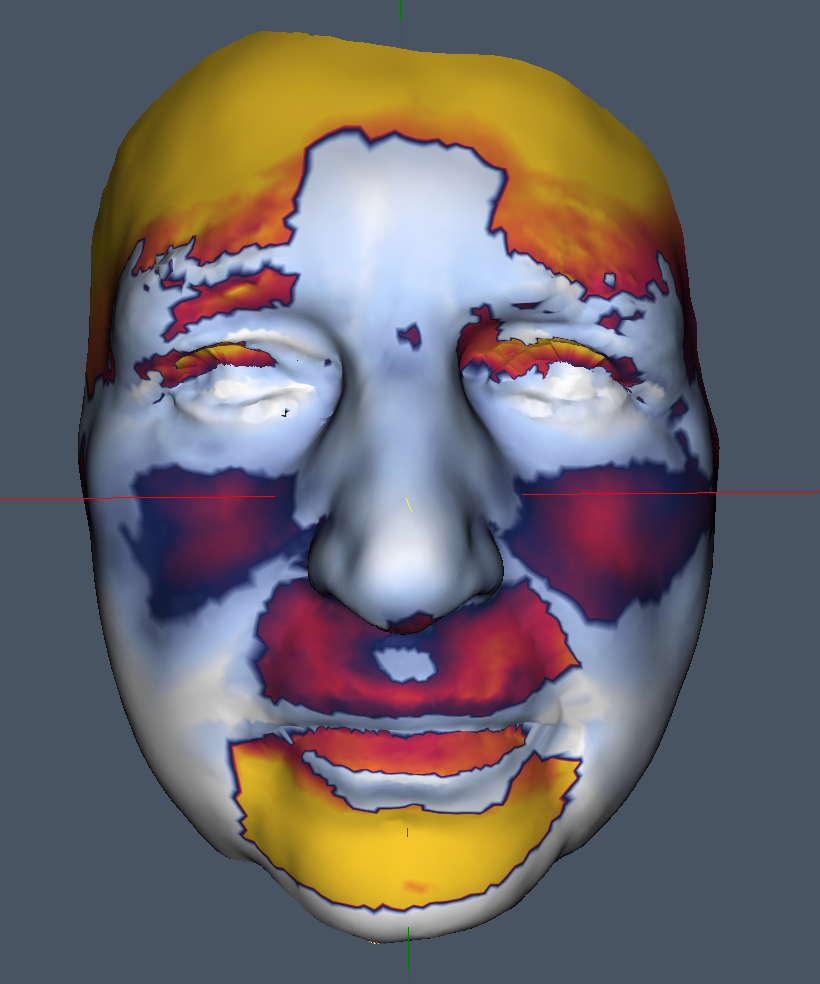
\includegraphics[width=0.5\textwidth]{./img/morpho-example01.PNG}
\caption{Morphome3cs - Vertex difference visualization}
\label{fig:morpho_example}
\end{figure}

Other approaches can be found for example in MeshLab (fig. \ref{fig:meshlab_example}) and CloudCompare (fig. \ref{fig:cloudcompare_example}). Both programs, however, also use only color-based visualizations. Both programs work with arbitrary triangle meshes and CloudCompare can also work with point clouds, register them and visualize the difference between them.

\begin{figure}[h]
\centering
	\begin{subfigure}{0.3\textwidth}
	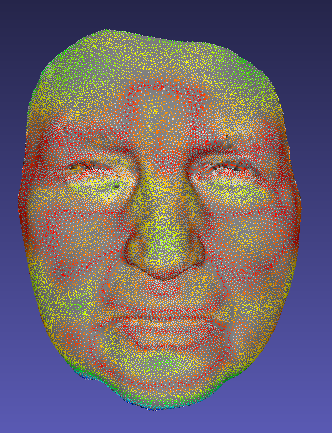
\includegraphics[width=\textwidth]{./img/meshlab-example01.PNG}
    \caption{MeshLab - Hausdorff Distance visualization}
    \label{fig:meshlab_example}
	\end{subfigure}
    \qquad
    \begin{subfigure}{0.3\textwidth}
	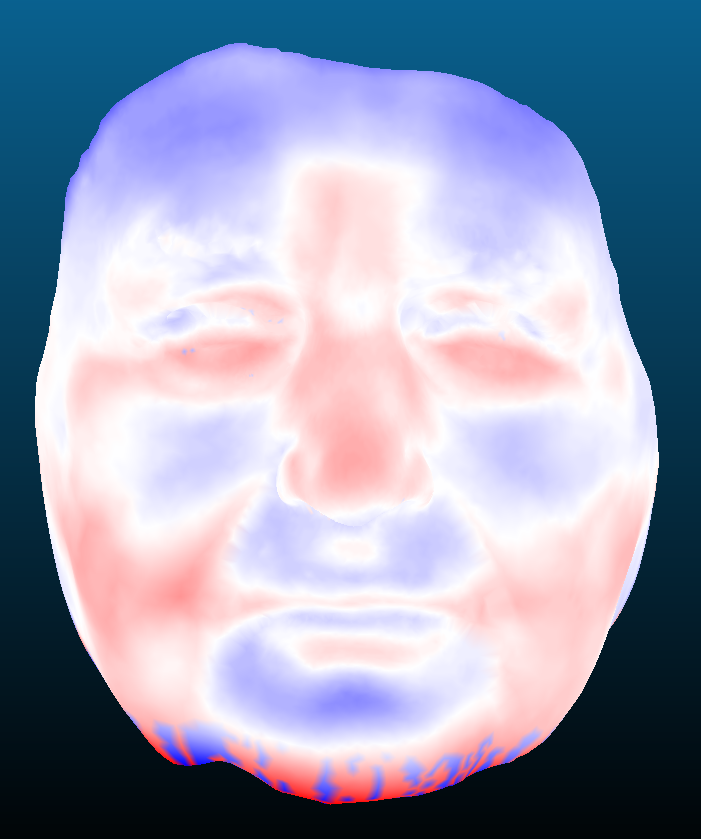
\includegraphics[width=\textwidth]{./img/cloudcompare-example01.PNG}
    \caption{CloudCompare - Vertex distance visualization}
    \label{fig:cloudcompare_example}
	\end{subfigure}
\caption{Visualizations in MeshLab and CloudCompare}
\end{figure}

\addtocounter{footnote}{-2}
\stepcounter{footnote}\footnotetext{Two triangle meshes are homologous if they have the same number of vertices and there is a one-to-one mapping between them. Vertices are numbered and vertex \(v_i \in Mesh_1\) corresponds to vertex \(v_i \in Mesh_2\).}
\stepcounter{footnote}\footnotetext{{\it Finite Element Surface Analysis}, captures the difference between corresponding triangle areas}
%%-----------------------------------------------------------------------------------------
%% SECTION
%%-----------------------------------------------------------------------------------------
\section*{Our Goal}

In order to overcome the limitations of the above visualizations, this thesis is looking to create arrow-based visualizations which will be able to display multidimensional information. We will also focus on the visual appearance of devised visualizations and their implementation in an experimental application. Lastly, a user study will be carried out to assess the quality of the new visualizations in various use cases. This study will serve as a basis for further development and potential incorporation of the visualizations into Morphome3cs.
%%-----------------------------------------------------------------------------------------
%% SECTION
%%-----------------------------------------------------------------------------------------
\section{Thesis Structure}

TODO

\chapter{Problem Analysis \& Solution}
\label{sec:analysis}

We will start by illustrating the input to our visualization problem.

Our input are two homologous triangle meshes which are to be compared. In order to clearly distinguish between these two meshes, we will call one of them the {\it primary mesh} and the other one will be the {\it reference mesh}. The mesh which carries the visualization is always the {\it primary mesh}. For example, Fig. \ref{fig:morpho_example} shows a {\it primary mesh}. The visualization demonstrates how different this {\it primary mesh} is from its {\it reference mesh}.

For the purposes of our arrow-based visualization technique, it is suitable to use difference metrics which can be represented by 3D vectors because these can be directly rendered as arrows. We will restrict ourselves to corresponding vertex distance because this metric used in Morphome3cs suffers from information loss when visualized using only colors. In addition to that, we will also include corresponding vertex distance projected into surface normal despite the fact that this metric only has one dimension. We will use it to compare arrow-based and color-based visualizations. Other metrics can be easily added if needed.

After a difference metric is computed, it is placed as a 3D vector in the corresponding vertex of the {\it primary mesh}. For a better understanding, here is the meaning of such a representation in case of both chosen metrics:

\begin{itemize}
\item For corresponding vertex distance, a vector is placed in the vertex of the {\it primary mesh} and if both meshes were overlaid, its apex would lie in the corresponding vertex of the {\it reference mesh}. This is therefore the most straightforward difference metric and it carries information in multiple dimensions, namely tangential difference and normal difference.
\item For corresponding vertex distance projected into surface normal, the situation is largely similar, only the metric has lost the dimension of tangential difference and is only represented by a single number. When a unit surface normal is multiplied by this number it yields our vector placed in a vertex of the {\it primary mesh}.
\end{itemize}

We will split the vectors into two groups. Vectors which have an acute angle with the positive surface normal will be said to point {\it outwards} and all other vectors will be said to point {\it inwards} (see Fig. \ref{fig:input}). This differentiation will become more meaningful when the meshes in question are for example human faces or other enclosed objects which are very common in geometric morphometrics.

\begin{figure}[h]
\centering
\def\svgwidth{\textwidth}
\input{./illustrations/input_illustration.pdf_tex}
\caption[Input Illustration]{A simplified schema of difference metric vectors. Yellow and blue arrows represent corresponding vertex distance, whereas red arrows show how the distance is projected into surface normal. Yellow arrows point {\it outwards} and blue arrows point {\it inwards}. Notice that all arrows are placed in the {\it primary mesh} and point towards the {\it reference mesh}.}
\label{fig:input}
\end{figure}

To summarize, we are now working with a {\it primary mesh} containing vectors in all its vertices and we are looking for a way to visualize these vectors using an arrow-based visualization. See Fig. \ref{fig:input} for a schema of this situation.

%%-----------------------------------------------------------------------------------------
%% SECTION
%%-----------------------------------------------------------------------------------------
\section{Seeing Mesh Difference as a Vector Field}

If all vectors were drawn directly onto the {\it primary mesh}, the visualization would become too cluttered (see Fig. \ref{fig:meshdiff_unclustered}). We also need a way to group similar vectors together to provide a more global difference visualization which existing color-based visualizations described in the introduction are incapable of.

\begin{figure}[h]
\centering
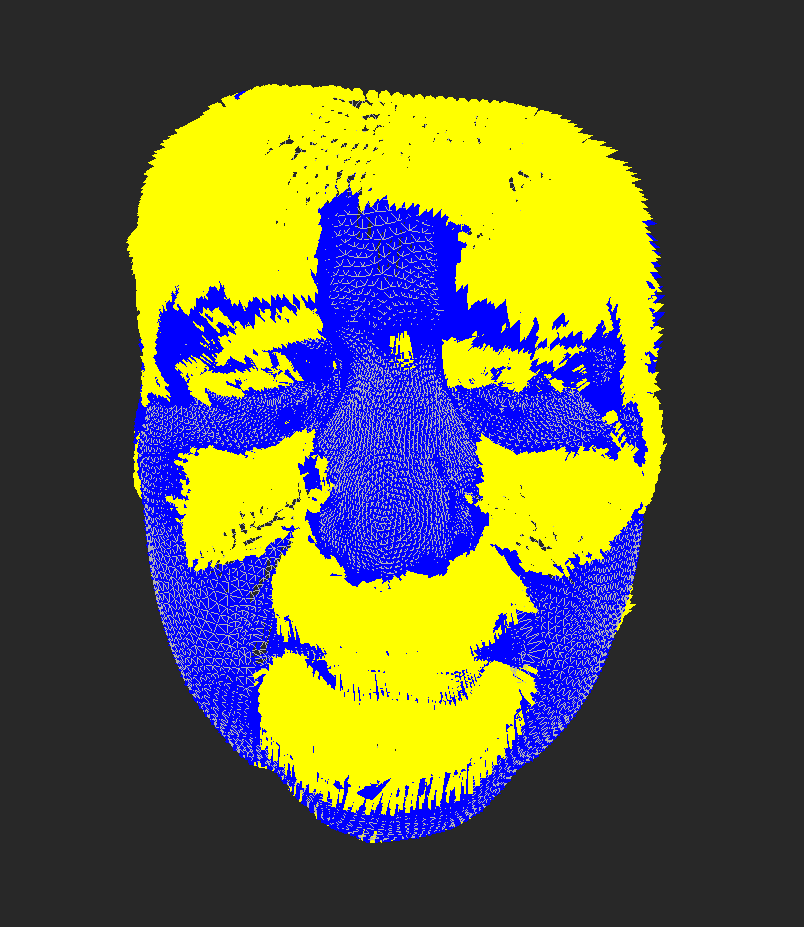
\includegraphics[width=0.5\textwidth]{./img/meshdiff-unclustered_arrows-single.png}
\caption[MeshDiff - Vertex distance visualized by unclustered arrows]{MeshDiff - Vertex distance visualized by unclustered arrows}
\label{fig:meshdiff_unclustered}
\end{figure}

One way to solve this problem is to devise a simple abstraction and use tools available for this abstraction.

Vectors saved in the vertices of a triangle mesh form a discrete bounded vector field. Visualization of discrete vector fields is a very active research area with applications in engineering, molecular modelling and computational fluid dynamics. There exist many scientific papers studying this topic, such as \citet{Telea99}, \citet{Garcke00}, \citet{Du04} or \citet{Peng12}.

Drawing inspiration from these papers we will employ a clustering technique to reduce the number of vectors and subsequently visualize this reduced information.

To summarize again, we are now visualizing a discrete bounded vector field.

%%-----------------------------------------------------------------------------------------
%% SECTION
%%-----------------------------------------------------------------------------------------
\section{Vector Field Clustering}

Clustering in general is a very subjective task (see Fig. \ref{fig:clustering_subjectivity}) and there are numerous approaches to clustering available. For this reason we present an overview of clustering techniques used in vector field visualization to gain a better understanding of which technique might best suit our purposes and why.

\begin{figure}[h]
\centering
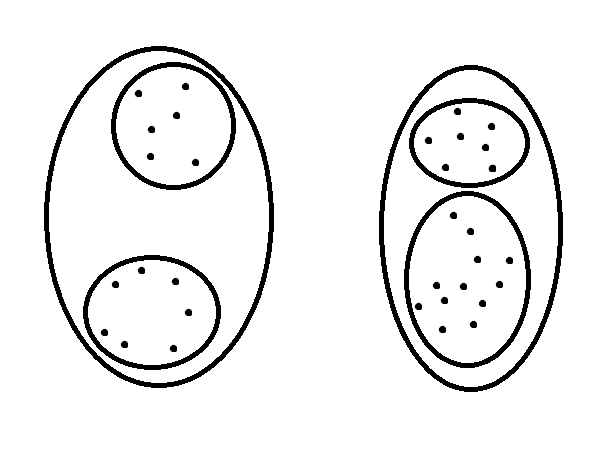
\includegraphics[width=0.6\textwidth]{./img/clustering_subjectivity.png}
\caption[The subjectivity of clustering]{The subjectivity of clustering - are there two or four clusters in the image?}
\label{fig:clustering_subjectivity}
\end{figure}

%%-----------------------------------------------------------------------------------------
\subsection{Overview of Vector Field Clustering Methods}

\citet{Telea99} use hierarchical clustering\footnotemark where neighboring clusters with the lowest clustering error are merged first. Each cluster has a representative vector and during the merge, the weighted average of the two vectors is computed and assigned to the newly formed cluster. In order to compute the clustering error, the paper introduced elliptic iso-error contours\footnotemark. This clustering method is primarily aimed at 2D rectilinear vector fields but can be also used in 3D when the error function is modified appropriately. It is possible to use up to seven parameters to configure the clustering.

\addtocounter{footnote}{-2}
\stepcounter{footnote}\footnotetext{Hierarchical clustering, also called bottom-up clustering, starts with each data point representing an elementary cluster. In each step of the algorithm, two clustering candidates are found from the available clusters according to certain criteria and subsequently merged. Hierarchical clustering creates a binary tree, also called a dendrogram, where each node represents a cluster and has two children from which it was created. Arbitrary number of clusters covering the whole data set can then be obtained by taking roots of disjoint subtrees which, when combined, contain all the leaves of the dendrogram. See Fig. \ref{fig:telea-hierarchical_clustering}.}
\stepcounter{footnote}\footnotetext{Clustering error in \citet{Telea99} is computed by measuring the "distance" between the representative vectors \(v, w\) of the two clusters. The elliptic iso-error contour is an ellipse which has a center on the line determined by \(v\) and intersects the apex of \(w\). All vectors \(w'\) which share the same ellipse have the same "distance" from \(v\). The shape of the ellipse and the location of its center can be controlled by parameters. See Fig. \ref{fig:telea-hierarchical_clustering}.}

\begin{figure}[h]
\centering
	\begin{subfigure}{0.5\textwidth}
	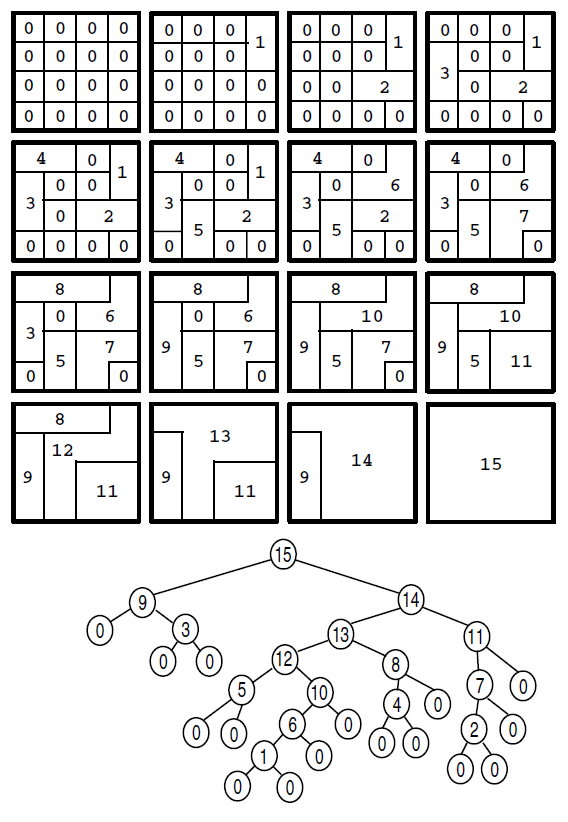
\includegraphics[width=\textwidth]{./img/telea-hierarchical_clustering.PNG}
    \caption{Various clusterings of a data set and the corresponding dendrogram}
	\end{subfigure}
    \qquad
    \begin{subfigure}{0.3\textwidth}
	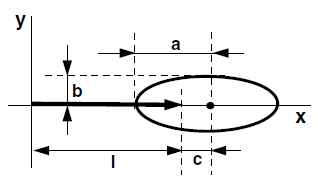
\includegraphics[width=\textwidth]{./img/telea-ellipse-params.PNG}
    \caption{The ellipse and its parameters.}
    
    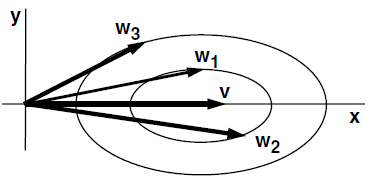
\includegraphics[width=\textwidth]{./img/telea-ellipse-vectors.PNG}
    \caption{The iso-error contours of multiple vectors}
	\end{subfigure}
\caption[The illustration of clustering in \citet{Telea99}]{The illustration of clustering in \citet{Telea99}}
\label{fig:telea-hierarchical_clustering}
\end{figure}

\citet{Garcke00} use a continuous clustering method\footnotemark based on the physical model of \citet{CahnHilliard58} which is used to describe phase separation and coarsening in binary alloys. This model is applied to vector field data which results in a diffusion problem rather than a splitting and merging problem. Their algorithm also assumes an either 2D or 3D rectilinear grid.

\footnotetext{In continuous clustering methods, there is no notion of merging or splitting in each step of the algorithm. Instead, ``a continuous scale of successively coarser cluster sets" is created.}

\citet{Du04} use iterative clustering\footnotemark where Voronoi regions\footnotemark are created around the initial cluster centers and a distance function is applied to each of them. The set of clusters which has the lowest value of the distance function is selected as the final cluster set. This method works with 2D and 3D rectilinear vector fields and can be influenced by two parameters and by the distribution of the initial clusters.

\addtocounter{footnote}{-2}
\stepcounter{footnote}\footnotetext{Iterative clustering algorithms start by assigning the data points to a given number of clusters in a random way or by using a clustering approximation. In each step, the clustering error of all clusters is computed and data points are reassigned in a way which decreases the overall clustering error.}
\stepcounter{footnote}\footnotetext{Voronoi diagram is a partitioning of a plane into regions. The partitioning is done by selecting some initial points as seeds. Then a region is formed around each seed in such a way that a point \(p\) of the plane belongs to the region of seed \(s\) if and only if \(d(p, s') \geq d(p, s) \forall s' \text{ seeds, such that } s' \neq s\).}

\citet{Peng12} use hierarchical clustering similar to \citet{Telea99} with the difference that the clustering is computed on a GPU by encoding a given static view of the vector field into a rasterized image. The computation is then done for this specific image. In order to obtain the clustering error of clusters \(C_1, C_2\), a very simple formula is used:

\begin{equation} \label{eq:clustering_error}
\bm{e}(C_1,C_2) = k_d \cdot \frac{d_{C_1C_2}}{d_{max}} + k_v \cdot \frac{v_{C_1C_2}}{v_{max}} + k_\alpha \cdot \frac{\alpha_{C_1C_2}}{\alpha_{max}} + k_m \cdot \frac{m_{C_1C_2}}{m_{max}}
\end{equation}

where \(k_d + k_v + k_\alpha + k_m = 1\) are weight coefficients. The other components are the following:

\begin{itemize}
\item \(d_{C_1C_2}\) is the Euclidean distance between the positions of the representative vectors of the clusters. The maximum distance \(d_{max}\) is the length of a diagonal of the geometry's bounding box
\item \(v_{C_1C_2}\) is the difference between the lengths of the representative vectors and \(v_{max}\) is the largest length in the whole data set.
\item \(\alpha_{C_1C_2}\) is angle between the representative vectors. The maximum angle is \(\alpha_{max} = 180^\circ\)
\item \(m_{C_1C_2}\) is the sum of the mesh resolutions of the two clusters. \(m_{max}\) is the largest value of \(m\) in the whole data set.
\end{itemize}

The mesh resolution component also differentiates this approach from all others because it represents an approximation of the density of the underlying mesh in a given local area. Including it in the error formula assigns higher error to dense clusters which results in a larger amount of clusters (higher precision) in dense areas of the mesh and a smaller amount of clusters (lower precision) in sparse areas of the mesh. This method is therefore aimed at non-rectilinear 3D vector fields. It has five parameters for user configuration (four weights and the number of clusters to be retrieved from the dendrogram).
%%-----------------------------------------------------------------------------------------
\subsection{Selection Criteria for Our Clustering Method}

For our visualization purposes, we will utilize fragments of the presented clustering methods and introduce certain modifications to accommodate our needs. Here are the criteria for choosing our clustering method:

\begin{itemize}
\item Suitability for the specifics of our vector field
\item Simplicity
\item Ease of user configuration
\end{itemize}

Methods which are suitable for our specific vector field (i.e. a triangle mesh with a vector in each vertex) will help us tailor the clustering process and achieve better results. 

Simple methods will allow us to quickly obtain a baseline which will help us to decide which modifications will improve the algorithm in our conditions. 

Lastly, the ease of user configuration will make our algorithm user-friendly and therefore it will increase the adoption rate.

%%-----------------------------------------------------------------------------------------
\subsection{Our Clustering Method}

We will now describe our clustering method.

\subsubsection{Clustering Algorithm}
\label{sec:analysis_clustering_algorithm}

The preference of hierarchical clustering over other mentioned clustering methods is justified by its simplicity and also the fact that a dendrogram is created during this clustering. This will allow us to quickly react to user requests for various cluster counts with given clustering parameters. Hierarchical clustering will thus make our approach user-friendly. We will, however, introduce one optional condition as to which clusters can be merged together. Our clustering candidates will not only have to be neighbors (as in \citet{Telea99}) but their representative vectors will both have to point either {\it inwards} or {\it outwards} because this distinction may be of importance to the user. On the other hand, we leave this condition as optional because the resulting dendrogram is not a tree but a forest instead. This may result in undesirable artifacts in the visualization because for certain cluster counts, the clustering will not cover the whole data set. See Fig. \ref{fig:forest_dendrogram} for an illustration.

\begin{figure}[h]
\centering
\def\svgwidth{\textwidth}
\input{./illustrations/forest_dendrogram.pdf_tex}
\caption[Forest Dendrogram]{An illustration of clustering with the optional condition enabled and the resulting dendrogram.}
\label{fig:forest_dendrogram}
\end{figure}

We are not going to use the GPU-based approach to clustering computation from \citet{Peng12} because it does not allow the user to view the final visualization from varying angles in real time. In order to support interactive visualization viewing, we will store our vector field in memory and compute the clustering on the whole field in one process instead (as in \citet{Telea99}).

\subsubsection{Clustering Error Function}

We will use the error function presented in \citet{Peng12} (see Eq. \ref{eq:clustering_error}) because it is the only one which assumes vector fields on other than rectilinear grids. Its mesh resolution component makes it suitable to use in the clustering of vector fields on triangle meshes. The function is also simpler and more easily scalable than the elliptic iso-error contours presented in \citet{Telea99} which lead to cube root equations in 3D.

\subsubsection{Cluster Merging}

Besides clustering error computation, merging is the second crucial part of a hierarchical clustering algorithm. In the clustering of vector fields, a representative vector is usually assigned to a newly formed cluster. In our case, this shall be a weighted average of the representative vectors of the child clusters where the weight will be the geometrical area of the given cluster. Geometrical area is a better metric for cluster size than data point count because our underlying triangle mesh is expected to be of varying density.

\subsubsection{Summary}

Our clustering method will use the hierarchical algorithm and CPU-based clustering computation from \citet{Telea99} with the added optional condition of merging only clusters whose representative vectors both point in the same direction - either {\it inwards} or {\it outwards}. We will use the error function from \citet{Peng12} (see Eq. \ref{eq:clustering_error}). Merging of two clusters will be done by computing the area-weighted average of their representative vectors and assigning the resulting vector to the newly formed cluster.

After the clustering step, we are visualizing a set of clusters, each of which has a representative vector which encodes a difference metric averaged across the whole cluster.
%%-----------------------------------------------------------------------------------------
%% SECTION
%%-----------------------------------------------------------------------------------------
\section{Proposed Visualizations}
\label{sec:analysis_visualizations}

Here we present the descriptions of new visualizations. One of them is arrow-based as was our goal and the rest are complementary visualizations leveraging the clustering process in order to enhance the visual appearance and clarity of existing visualization techniques.

%%-----------------------------------------------------------------------------------------
\subsection{Arrows}
\label{sec:arrow_vis}

Once a clustering of a vector field is obtained, representative vectors of all clusters are visualized using 3D arrows. For this purpose we have prepared a simple 3D model of an arrow (see Fig. \ref{fig:arrow_model}) which is copied to the scene at a specific position, angle and scale given by the representative vector and the cluster it belongs to.

\begin{figure}[h]
\centering
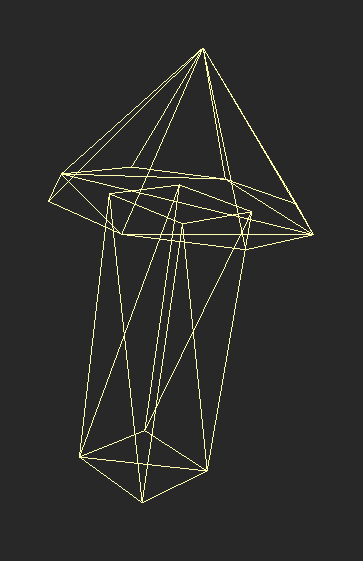
\includegraphics[width=0.3\textwidth]{./img/8sided_arrow.PNG}
\caption[Arrow Model]{Wireframe view of the 3D arrow model}
\label{fig:arrow_model}
\end{figure}

The length of the representative vector influences the length of the 3D arrow. Because the values of the metric can be very close to zero and because their value range is not generally very large, we have decided to set a certain minimum scale and maximum scale, which are adjustable by the user, and map the metric values (vector lengths) to the interval between them. In general, such an approach gives a more visually pleasing and clearer results, especially when the interval is chosen to be large enough.

The scale of the 3D arrows also reflects the geometrical area of the clusters. The larger the clusters are, the thicker the arrows. Areas are again mapped to a user-defined interval for a clearer result. Large clusters are usually important because they represent a general trend in a given area and users should be able to see them more easily and also distinguish them from less important clusters.

Lastly, and most importantly, the direction of the representative vector is reflected directly in the direction of the 3D arrow. In addition to that, Arrows pointing {\it inwards} can have a different color than arrows pointing {\it outwards} to make their differentiation easier for the user.

We have therefore managed to encode three-dimensional information into our visualization.

\begin{figure}[h]
\centering
	\begin{subfigure}{0.3\textwidth}
	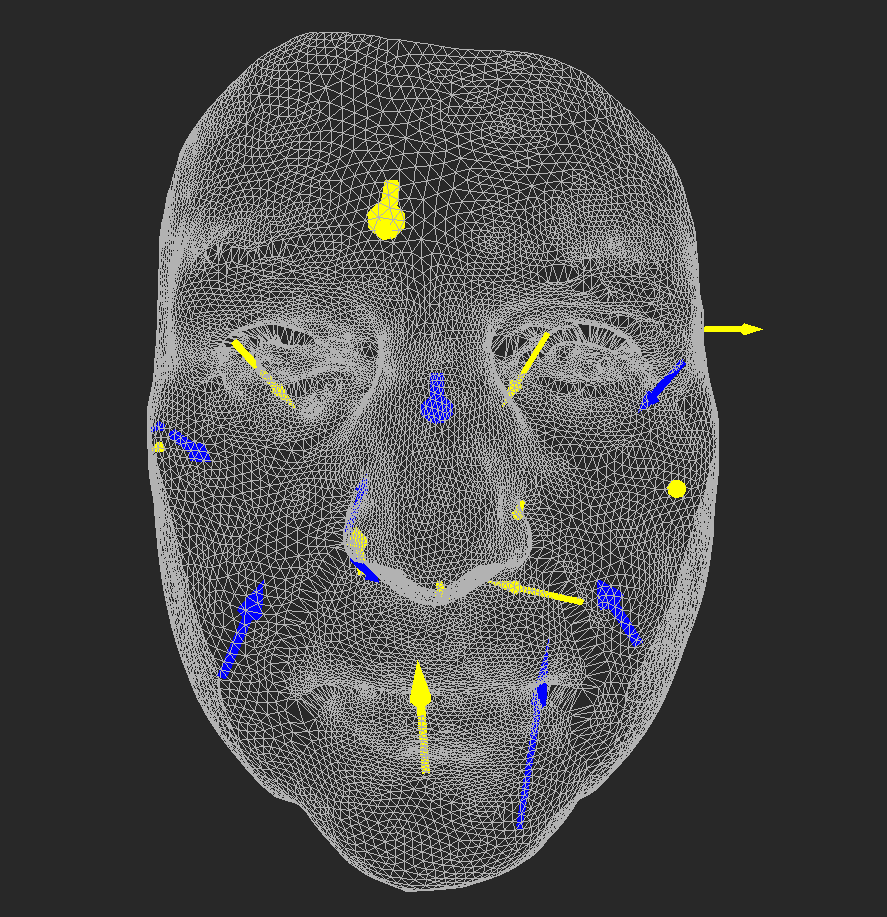
\includegraphics[width=\textwidth]{./img/meshdiff-arrows-interval0_5-5-count20-single.png}
    \caption{Smallest height \& width scale: \(0.5\); largest height \& width scale: 5; cluster count: 20}
    \label{fig:meshdiff_arrows_5-20}
	\end{subfigure}
    \qquad
    \begin{subfigure}{0.3\textwidth}
	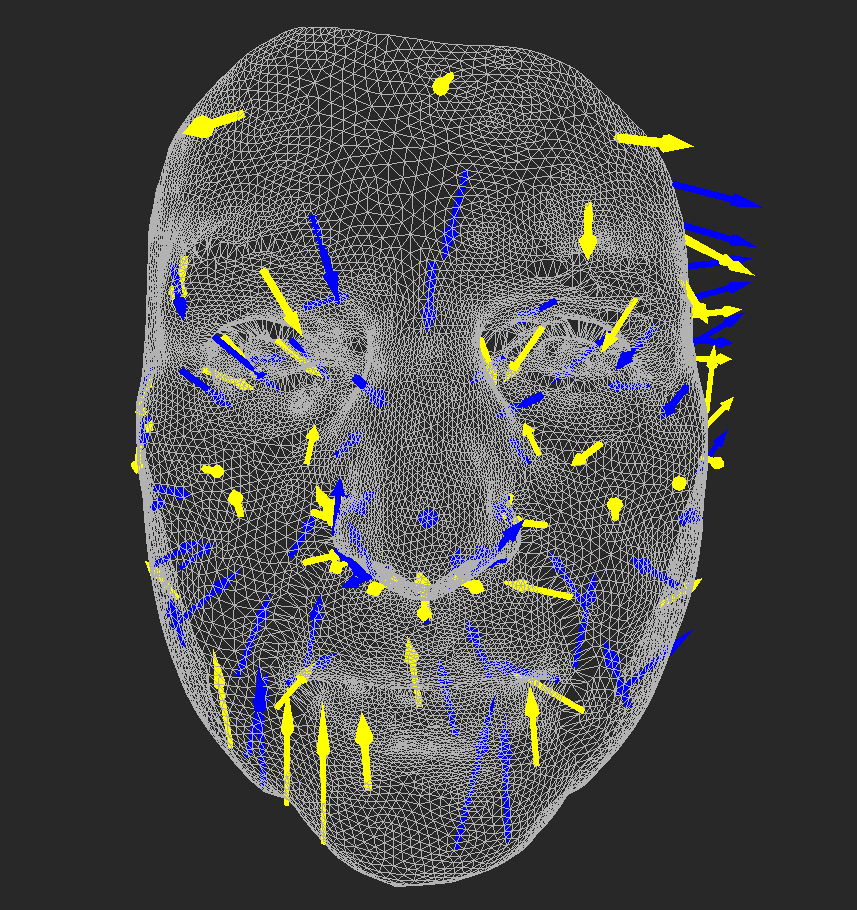
\includegraphics[width=\textwidth]{./img/meshdiff-arrows-interval0_5-5-count125-single.png}
    \caption{Smallest height \& width scale: \(0.5\); largest height \& width scale: 5; cluster count: 125}
    \label{fig:meshdiff_arrows_5-125}
	\end{subfigure}
    
    \begin{subfigure}{0.3\textwidth}
	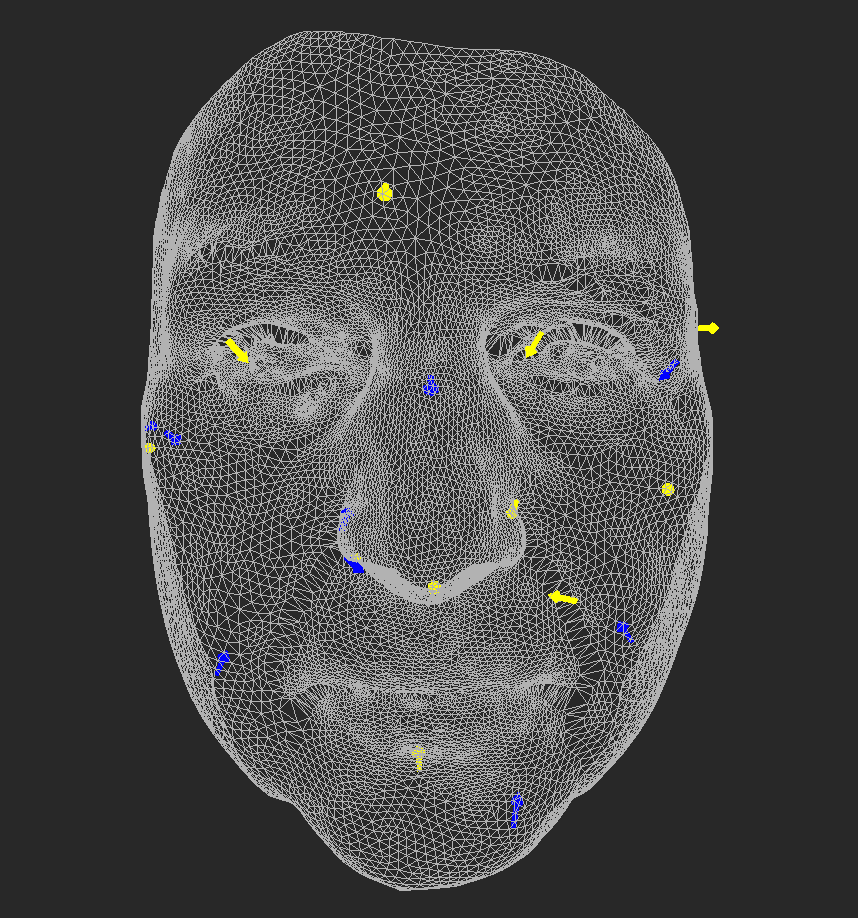
\includegraphics[width=\textwidth]{./img/meshdiff-arrows-interval0_5-1-count20-single.png}
    \caption{Smallest height \& width scale: \(0.5\); largest height \& width scale: 1; cluster count: 20}
    \label{fig:meshdiff_arrows_1-20}
	\end{subfigure}
    \qquad
    \begin{subfigure}{0.3\textwidth}
	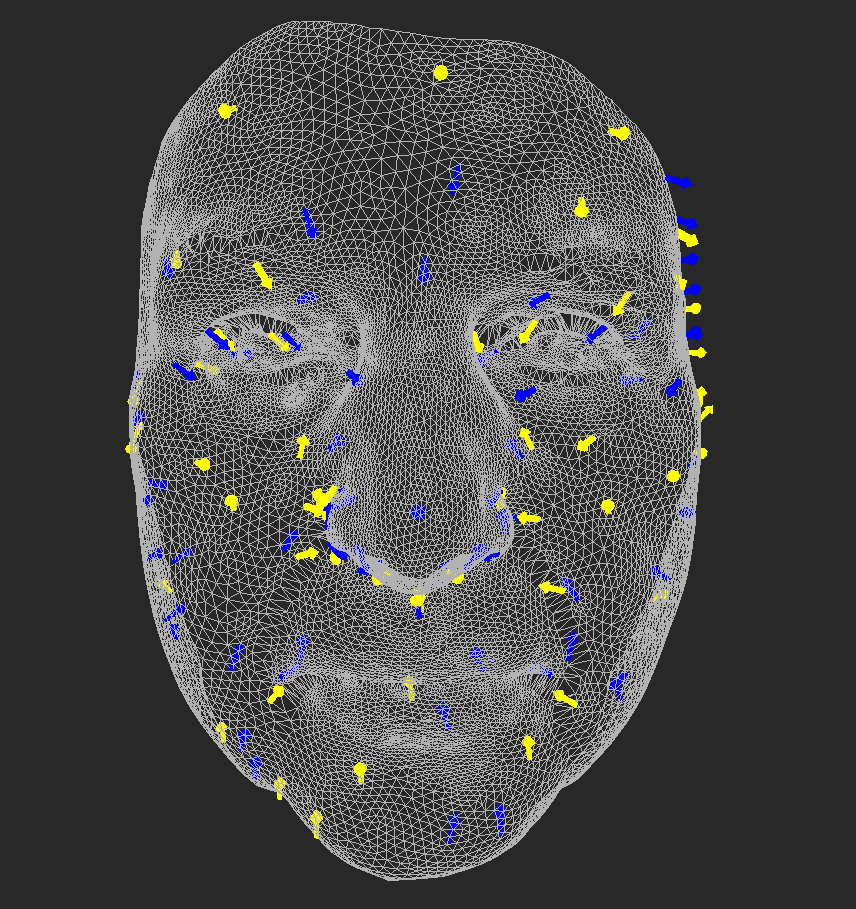
\includegraphics[width=\textwidth]{./img/meshdiff-arrows-interval0_5-1-count125-single.png}
    \caption{Smallest height \& width scale: \(0.5\); largest height \& width scale: 1; cluster count: 125}
    \label{fig:meshdiff_arrows_1-125}
	\end{subfigure}
\caption[MeshDiff - Arrow visualizations with various parameter settings]{MeshDiff - Arrow visualizations with various parameter settings}
\end{figure}

\subsubsection{Expected Performance}

Arrow visualizations combined with clustering are expected to perform well in answering questions about general trends in large parts of the mesh. They are also expected to perform considerably better than color-based visualizations when asking about the direction of the difference, which is particularly important in cases when the difference has a very small angle with the surface of the mesh.
%%-----------------------------------------------------------------------------------------
\subsection{Cluster Color}
\label{sec:analysis-color}

Next, we introduce two color visualizations of clusters: random and metric-based.

Both of these visualizations need to be aware of which mesh vertices belong to a given cluster. Then either a random color is assigned to all vertices in a given cluster or a color based on the length of the representative vector of the cluster is assigned. The former case is basically the original color visualization of a metric, only applied to clusters.

We propose two modes of assigning the color to the vertices based on metrics, the relative mode and the absolute mode. In both modes, a distinct user-defined color hue is assigned to clusters whose representative vectors point {\it inwards} and {\it outwards}. Also, the metric value here is the length of the associated vector. What differentiates the two modes is the shade assigned to clusters of specific metric value.

In the relative mode, the highest and lowest metric values are evaluated first. The lowest value receives black color and the highest value receives the brightest user-defined color. All other values are mapped to this interval and receive a color which is a proportional mixture of the user-defined color and black.

In the absolute mode, black color is assigned to cluster of zero metric value and the brightest color is assigned to clusters of metric value higher or equal than a user-defined value. This allows the user to compare across several visualizations and determine the absolute value of the difference metric more easily.

\begin{figure}[h]
\centering
	\begin{subfigure}{0.3\textwidth}
	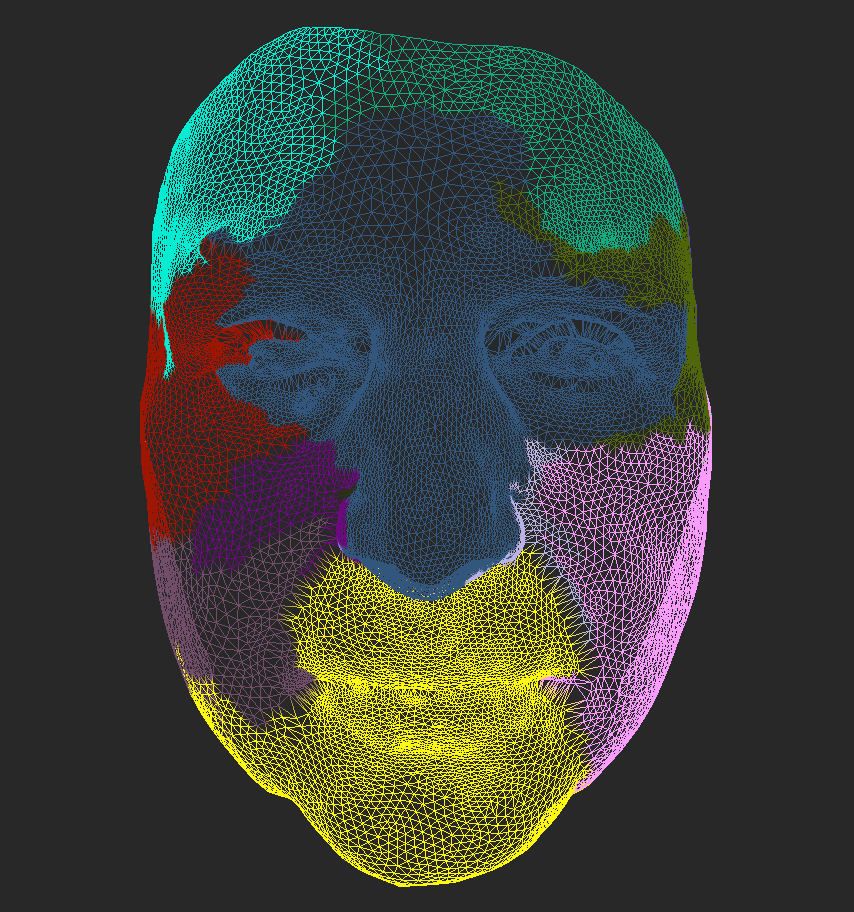
\includegraphics[width=\textwidth]{./img/meshdiff-clustercolor-random.PNG}
    \caption{Random cluster colors}
    \label{fig:meshdiff_clustercolor_random}
	\end{subfigure}
    \qquad
    \begin{subfigure}{0.3\textwidth}
	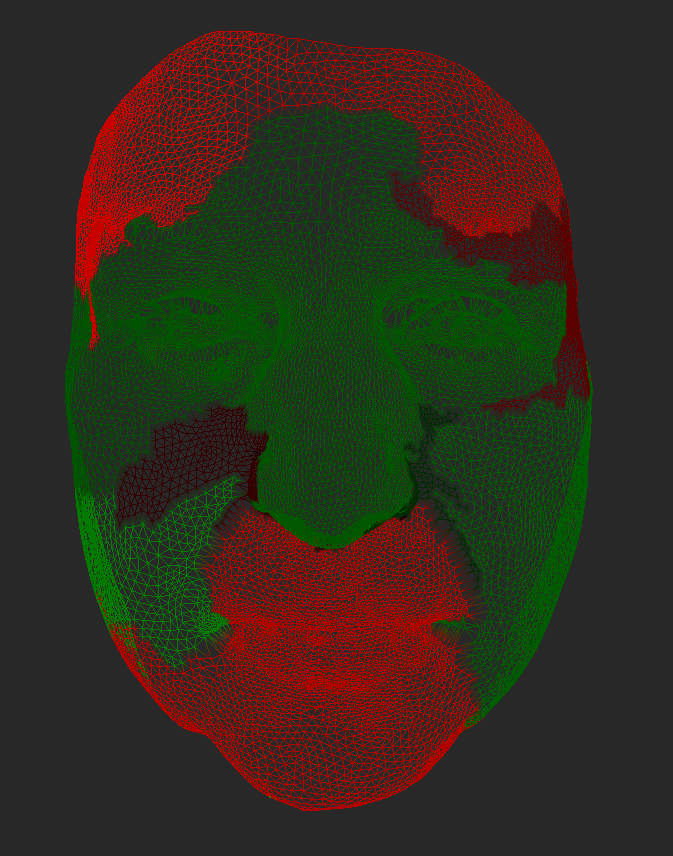
\includegraphics[width=\textwidth]{./img/meshdiff-clustercolor-metric.PNG}
    \caption{Metric-based cluster colors}
    \label{fig:meshdiff_clustercolor_metric}
	\end{subfigure}
    
\caption[MeshDiff - Cluster color visualizations]{MeshDiff - Cluster color visualizations}
\end{figure}

\subsubsection{Expected Performance}

Random cluster color is expected to be used for the purpose of configuring the clustering parameters as the size and the location of the clusters is clearly visible in this case.

Metric-based cluster color is expected to perform well in cases when we have found the most important differences using a more sophisticated visualization and want to present those using a visualization which is as clear as possible.
%%-----------------------------------------------------------------------------------------
\subsection{Thresholding}

For all types of metric-based visualizations including the original color-based ones we present thresholding. The thresholding is either applied to metric values which are too low or clusters whose area is too small. It acts as a high-pass filter and all visualization elements related to the metric or cluster which has not passed the thresholding is excluded from the result.

\begin{figure}[h]
\centering
	\begin{subfigure}{0.3\textwidth}
	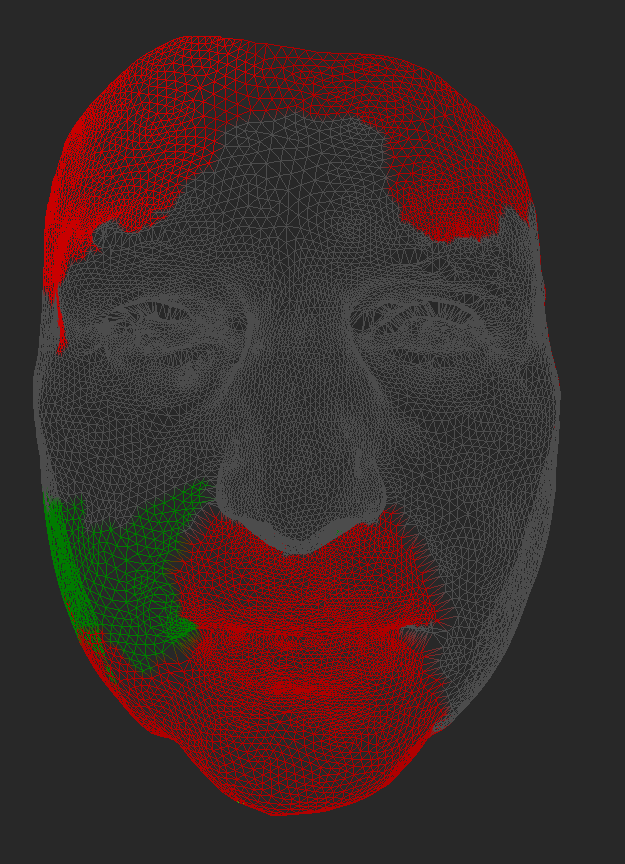
\includegraphics[width=\textwidth]{./img/meshdiff-thresholding-clustercolor-length3.PNG}
    \caption{Clusters with distance less than 3 grayed out}
    \label{fig:meshdiff_thresholding_clustercolor}
	\end{subfigure}
    \qquad
    \begin{subfigure}{0.3\textwidth}
	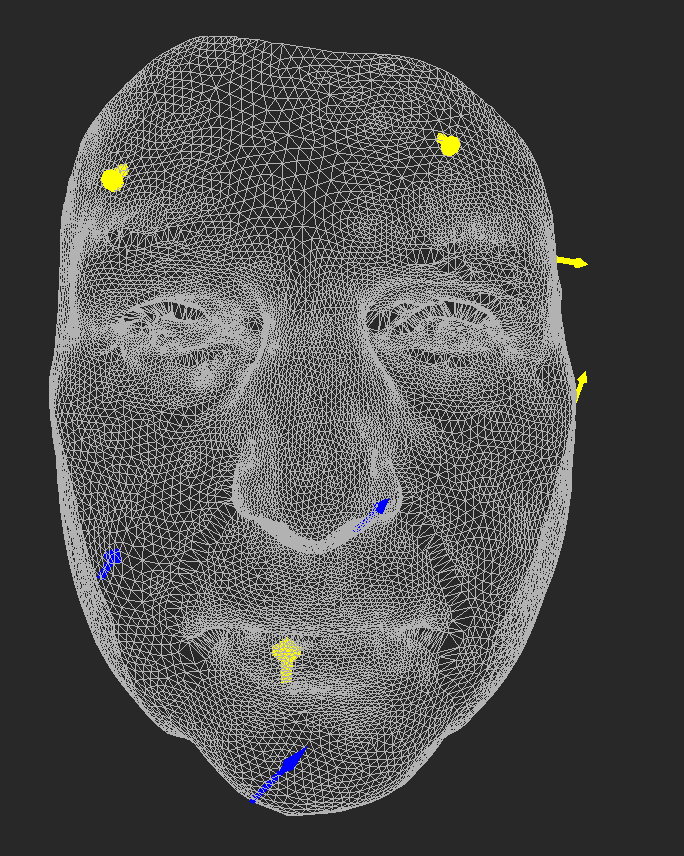
\includegraphics[width=\textwidth]{./img/meshdiff-thresholding-arrows-length3.PNG}
    \caption{Arrows for cluster with distance less than 3 excluded}
    \label{fig:meshdiff_thresholding_arrows}
	\end{subfigure}
    
\caption[MeshDiff - Thresholded visualizations]{MeshDiff - Thresholded visualizations}
\end{figure}

\subsubsection{Expected Performance}

Thresholding is expected to enhance the effect of metric-based cluster color visualizations by performing very well when segmenting and emphasizing a previously discovered difference which is important to the user. It is also expected to help answer questions about the largest differences between two meshes.
%%-----------------------------------------------------------------------------------------
\subsection{Combined Visualizations}

The last visualization type presented in this thesis is the combination of color and arrow visualizations.

\begin{figure}[h]
\centering
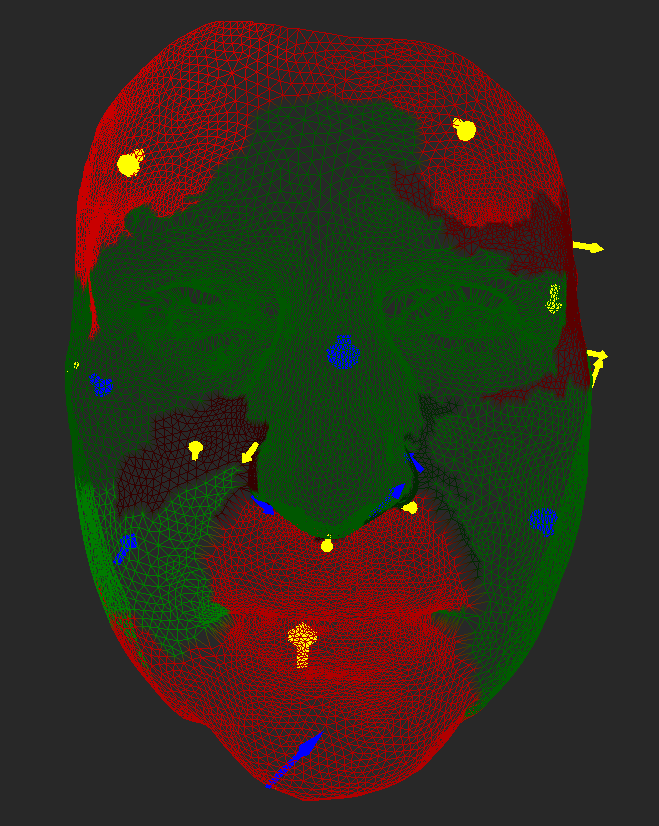
\includegraphics[width=0.5\textwidth]{./img/meshdiff-combination.PNG}
\caption[MeshDiff - Combined visualization]{MeshDiff - Combined visualization}
\label{fig:meshdiff_combination}
\end{figure}

\subsubsection{Expected Performance}

Combined visualizations complement each other in areas when only one visualization is not sufficiently clear. Color visualization is expected to highlight the dimension of the metric we are interested in the most, for example vertex distance magnitude, while arrow visualization is expected to carry other dimensions like direction and cluster size. This method is expected to have a good balance between clarity and information richness.
%%-----------------------------------------------------------------------------------------
%% SECTION
%%-----------------------------------------------------------------------------------------
\section{The Effect of Clustering Parameters}
\label{sec:parameter_effect}

The function used for computing the clustering error (see eq. \ref{eq:clustering_error}) has four parameters:

\begin{itemize}
\item Direction weight
\item Position weight
\item Magnitude weight
\item Resolution weight
\end{itemize}

A specific configuration of these parameters can influence the outcome of the clustering process considerably. In general, setting one of them higher than others results in finer clustering in that dimension and coarser clustering in others. We will now describe the effect of each of the parameters in more detail.

%%-----------------------------------------------------------------------------------------
\subsection{Direction Weight}

High direction weight forms many small clusters in areas of high surface curvature and large clusters in flat areas. Therefore, it mostly captures the high-curvature changes of shape. Resulting clusters have uneven sizes.
%%-----------------------------------------------------------------------------------------
\subsection{Position Weight}

Setting the position weight higher than others results in clusters of even size where each of them represents the overall difference in a certain area regardless of the variety of directions and magnitudes in that area.
%%-----------------------------------------------------------------------------------------
\subsection{Magnitude Weight}

Magnitude weight can play a significant role when using the metric-based cluster color visualization because its high value will highlight iso-magnitude contours like in a geographical map. Such an approach can be useful when grouping and segmenting areas with a certain absolute value of the difference metric.
%%-----------------------------------------------------------------------------------------
\subsection{Resolution Weight}

High resolution weight prefers clustering in sparse areas of the mesh and will therefore increase the precision of the visualization in very dense areas. This effect partially complements high direction weight because high-curvature areas of triangle meshes are usually more dense in order for the high curvature to be captured well in the mesh.

\begin{figure}[h]
\centering
	\begin{subfigure}{0.3\textwidth}
	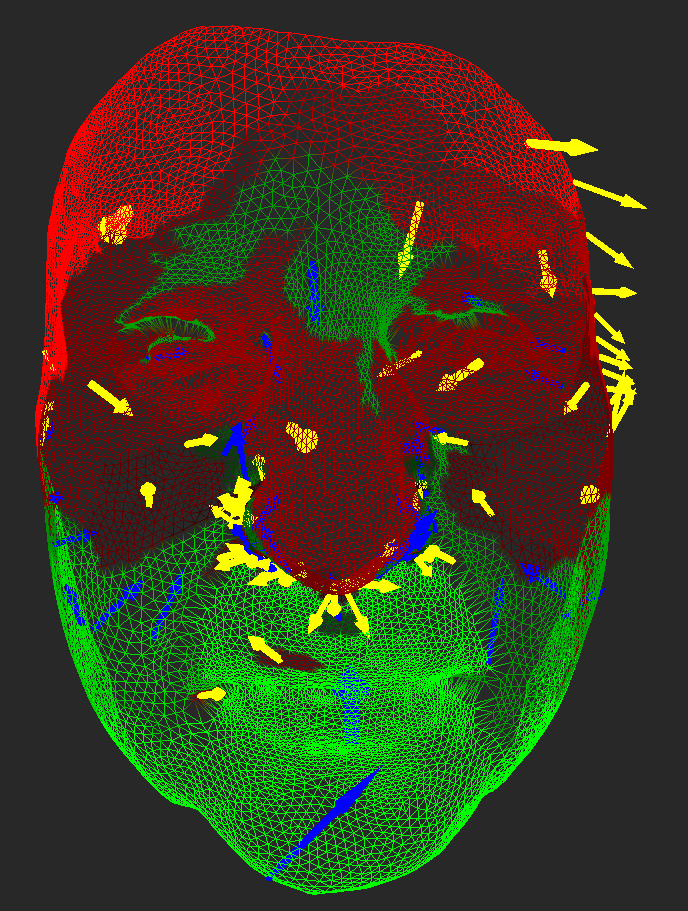
\includegraphics[width=\textwidth]{./img/meshdiff-high_direction.PNG}
	\caption{High direction weight}
	\label{fig:meshdiff_high_direction}
	\end{subfigure}
    \qquad
    \begin{subfigure}{0.3\textwidth}
	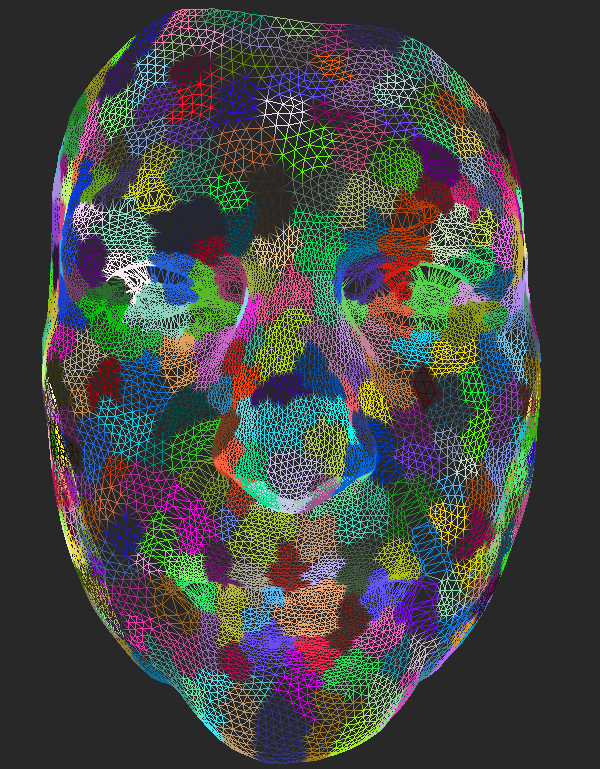
\includegraphics[width=\textwidth]{./img/meshdiff-high_position.PNG}
	\caption{High position weight}
	\label{fig:meshdiff_high_position}
	\end{subfigure}
    
    \begin{subfigure}{0.3\textwidth}
	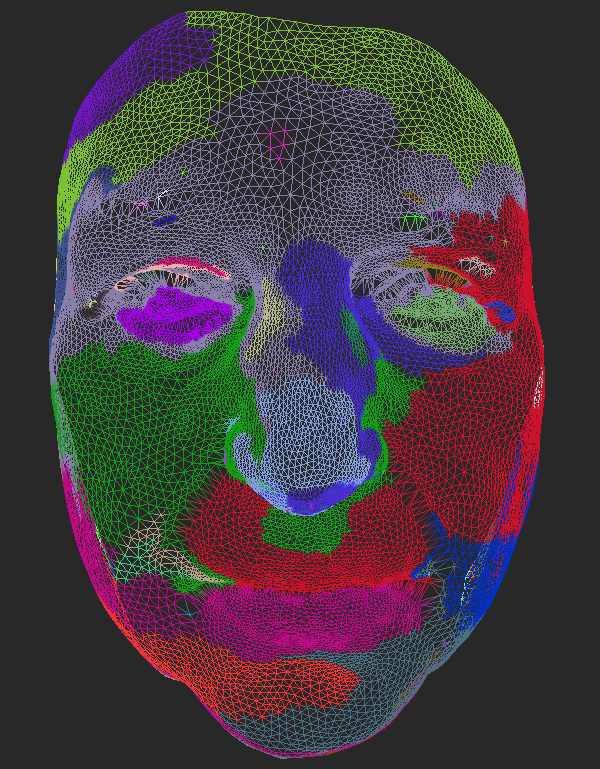
\includegraphics[width=\textwidth]{./img/meshdiff-high_magnitude.PNG}
	\caption{High magnitude weight}
	\label{fig:meshdiff_high_magnitude}
	\end{subfigure}
    \qquad
    \begin{subfigure}{0.3\textwidth}
	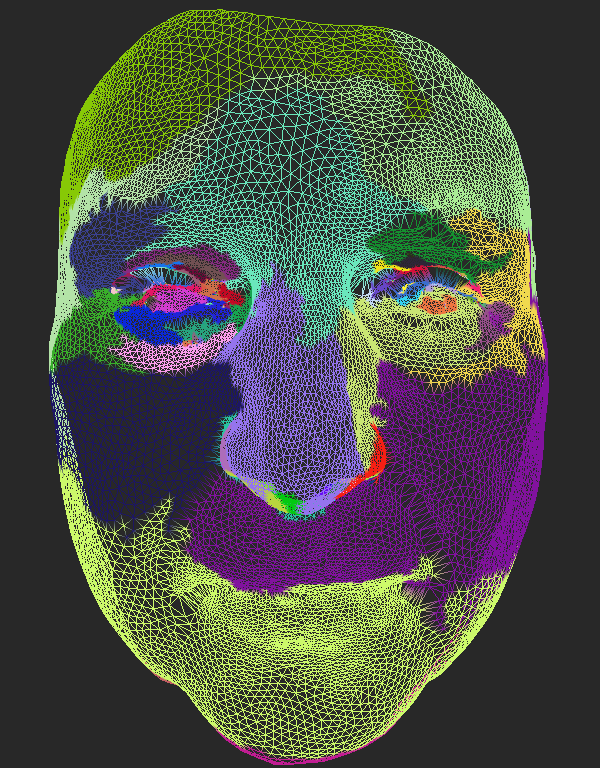
\includegraphics[width=\textwidth]{./img/meshdiff-high_resolution.PNG}
	\caption{High resolution weight}
	\label{fig:meshdiff_high_resolution}
	\end{subfigure}
\caption[MeshDiff - Various clustering parameter settings]{MeshDiff - Various clustering parameter settings}
\end{figure}
\chapter{Implementation}

In this chapter, we will delve into the implementation details of the presented visualizations applied in our experimental application called MeshDiff. We will also describe the overall architecture of MeshDiff.

%%-----------------------------------------------------------------------------------------
%% SECTION
%%-----------------------------------------------------------------------------------------
\section{Visualization Algorithm}
\label{sec:implementation_algorithm}

All presented visualizations share a common workflow (or algorithm) in MeshDiff. In this section, we will discuss the following parts of the workflow:

\begin{itemize}
\item Difference metric computation
\item Vector clustering
\item Vector visualization
\item Visualization output
\end{itemize}

First, however, we will describe the framework that the algorithm fits into and the internal representation of triangle meshes.

%%-----------------------------------------------------------------------------------------
\subsection{Algorithm Framework}
\label{sec:implementation-framework}

The core class of MeshDiff which encapsulates the visualization algorithm is called \verb+DiffVector+. The name of the class suggests that it is able to work with difference metrics which can be represented by a 3D vector. \verb+DiffVector+ is initialized by the {\it primary mesh} and the {\it reference mesh} and therefore only operates on these two specific meshes throughout its whole lifetime.

The main public methods of \verb+DiffVector+ are \verb+CreateVisualization()+ and \verb+BakeVisualization()+. \verb+CreateVisualization()+ is responsible for metric computation, data point clustering and the generation of a visualization. This visualization is then stored inside the \verb+DiffVector+ class and has to be obtained via the \verb+BakeVisualization()+ method.

This approach ensures that all intermediate results which are difficult to compute like data point clustering and visualization data can be stored inside the \verb+DiffVector+ class and quickly retrieved later if necessary. When a new visualization is created on the same pair of meshes, all intermediate results which can be reused are reused and only the ones which change are computed.

All visualization outputted from the \verb+BakeVisualization()+ class are in the form of triangle meshes which makes them easy to display, load and store using standard triangle mesh methods and formats. We will discuss this more in detail in section \ref{sec:implementation-visualizers-output} of this chapter.

%%-----------------------------------------------------------------------------------------
\subsection{Triangle Mesh Representation}
\label{sec:mesh_representation}

We are using an implementation of a triangle mesh boundary representation with a corner table which was presented in \citet{Corner03}. The implementation was written by Josef Pelikán. For brevity, we will refer to this representation as a {\it scene}\footnotemark.

\footnotetext{In this representation, we do not store the vertices of the triangle mesh but the corners of the triangles. The corner table then allows us to obtain the neighboring as well as opposite corners of a given corner and associated vertices in constant time. This makes traversing an arbitrary triangle mesh very simple and fast.}

We have added several methods to this implementation in order for us to be able to quickly obtain the list of neighbors of a given vertex and compute the geometrical area of clusters.

The pseudocode below describes the visualization workflow which will be further discussed in the following sections.

\begin{algorithm}[H]
\caption{CreateVisualization()}
\label{algo:create_vis}
\begin{algorithmic}[1]

\Require sceneP, sceneR, metricType, visualizerCol, visualizerArr, clusteringParams, visParams
\Statex
\If{required visualization exists}
	\State return READY;
\EndIf
\Statex \Comment Difference metric computation
\If{required metric value not available}
	\State arrows = GetArrows(sceneP, sceneR, metricType);
    \State clusteringObject = clusteringFactory(arrows, sceneP);
    \State currentMetricType = metricType;
\EndIf
\Statex \Comment Vector clustering
\State clusters = clusteringObject.GetClusters(clusteringParams);
\State currentClusteringParams = clusteringParams;
\Statex \Comment Vector visualization
\If{color visualization requested}
	\State colorVisP = visualizerCol.CreateVis(clusters, visParams);
    \State colorVisR = visualizerCol.CreateVisInv(clusters, visParams);
\EndIf
\If{arrow visualization requested}
	\State arrowVisP = visualizerArr.CreateVis(clusters, visParams);
    \State arrowVisR = visualizerArr.CreateVisInv(clusters, visParams);
\EndIf
\State currentVisParams = visParams;
\Statex
\State return READY;
\end{algorithmic}
\end{algorithm}

%%-----------------------------------------------------------------------------------------
\subsection{Difference Metric Computation}
\label{sec:analysis_metric}

Once the \verb+DiffVector+ class is initialized by the scenes of the {\it primary mesh} and the {\it reference mesh}, the configured difference metric can be computed.

The configuration is done via a parameter of the \verb+CreateVisualization()+ method. \verb+DiffVector+ remembers the current metric which it has computed and this determines whether metric data will be reused or whether a new set will be computed when \verb+CreateVisualization()+ is called.

As mentioned earlier, we have included two difference metrics in MeshDiff, both of which can be represented by a 3D vector:

\begin{itemize}
\item Corresponding vertex distance
\item Corresponding vertex distance projected into the surface normal
\end{itemize}

We have created a common representation for for both of these metrics called \verb+Arrow+ which encapsulates a 3D vector, its origin and other useful data and acts as an input to the clustering algorithm.

Here are the most important fields of \verb+Arrow+:

\begin{itemize}
\item \verb+Origin+ - a 3D vector representing the position of the vector metric and initially coincides with a {\it scene} vertex (this can change during the clustering process)
\item \verb+Direction+ - a 3D vector representing the metric itself
\item \verb+Orientation+ - tells whether the arrow points {\it inside} or {\it outside}
\item \verb+VertexHandle+ - if \verb+Origin+ coincides with a {\it scene} vertex, this is its index in the {\it scene} representation, otherwise it is -1
\end{itemize}

During this step, all corresponding vertices of both {\it scenes} are enumerated and for each pair, the configured metric is computed on the {\it primary scene} and relative to the {\it reference scene}. For example, consider a {\it primary scene} \(S_p\), a {\it reference scene} \(S_r\), vertices (vectors) \(\overrightarrow{v} \in S_p, \overrightarrow{w} \in S_r\) and a metric vector \(\overrightarrow{m}\). Then \(\overrightarrow{m_{vw}} = w - v\). This makes \(m_{vw}\) behave as described at the beginning of section \label{sec:analysis}.

\subsubsection{Output}

A list of \verb+Arrow+ instances indexed by the handles of the corresponding vertices in the {\it primary scene}.

%%-----------------------------------------------------------------------------------------
\subsection{Vector Clustering}
\label{sec:implementation_clustering}

As mentioned in \ref{sec:analysis_clustering_algorithm}, our clustering has multiple types. For the sake of consistency, we also introduce a third type, the empty clustering, which does not reduce the number of vectors in any way and can be used when no clustering is needed. Each clustering type has an associated class, all of which share a common interface.

Overall, there are three clustering types in MeshDiff:

\begin{itemize}
\item None
\item Simple (corresponds to clustering in \citet{Telea99})
\item Signed (merges only vectors pointing in the same direction, either {\it inwards} or {\it outwards})
\end{itemize}

The clustering type used in \verb+DiffVector+ is determined by a factory method passed to its constructor. \verb+DiffVector+ can therefore use the clustering without knowing its type and at the same time it is limited to using only one clustering type. Thanks to this, computed clusterings of multiple types can be saved at the same time and reused if needed. It is important to note that this reuse happens every time the user chooses to view a new visualization which differs from the previous one only in the number of clusters to be generated thanks to the dendrogram (see Fig. \ref{fig:telea-hierarchical_clustering}). The parameters of the clustering are passed directly to the \verb+CreateVisualization()+ method.

The clustering object also works in the \verb+CreateVisualization()+ where it is initialized with a list of \verb+Arrow+ instances from the previous step (\ref{sec:analysis_metric}), if those instances are newly computed (otherwise, the old clustering object is reused). First, it converts the \verb+Arrow+ instances (data points) to \verb+Cluster+ instances which are able to merge with other clusters and compute the clustering error given another \verb+Cluster+ instance. They also contain all the information needed for the visualization to be created. Here are the most important fields of \verb+Cluster+:

\begin{itemize}
\item \verb+Neighbors+ - a set of \verb+Cluster+ instances adjacent to the cluster
\item \verb+Level+ - marks the step of the clustering algorithm in which this cluster was created (low number also means low clustering error), it is illustrated in Fig. \ref{fig:telea-hierarchical_clustering}
\item \verb+RepresentativeArrow+ - an \verb+Arrow+ instance representing the metric value for this cluster
\item \verb+Size+ - the geometrical area of the cluster
\item \verb+LeftChild+ \& \verb+RightChild+ - \verb+Cluster+ instances out of which this cluster was created
\item \verb+PrimaryArrows+ - a list of all the original unclustered \verb+Arrow+ instances which are tied directly to the underlying mesh and which belong to this cluster
\end{itemize}

\verb+Cluster+ can be sorted and the sorting field is \verb+Level+.

After that, \verb+DiffVector+ passes clustering parameters and the required cluster count to the clustering object. The clustering object checks if it already has a clustering corresponding to the given parameters and if it does, it simply extracts the required number of clusters from the available dendrogram and returns them. This is how the extraction works when the dendrogram is a tree\footnote{In this case, merging candidates only have to be neighbors}:

\begin{algorithm}[H]
\caption{Cluster Extraction from a Tree}
\begin{algorithmic}[1]

\Require MaxHeap chosenClusters, requiredClusterCount
\Statex
\State chosenClusters.Clear();
\State chosenClusters.Insert(dendrogram root);
\State i = 0;
\While{i < requiredClusterCount}
	\State highestCluster = chosenClusters.ExtractMax();
    \State chosenClusters.Insert(highestCluster.LeftChild);
    \State chosenClusters.Insert(highestClusters.RightChild);
    \State i++;
\EndWhile
\Statex
\Return chosenClusters as list
\end{algorithmic}
\end{algorithm}

Here is the extraction algorithms for forest dendrograms\footnote{In this case, merging candidates have to be neighbors and their vectors must all point either {\it inwards}, or {\it outwards}}:

\begin{algorithm}[H]
\caption{Cluster Extraction from a Forest}
\label{algo:extraction_forest}
\begin{algorithmic}[1]

\Require MaxHeap chosenClusters, requiredClusterCount
\Statex
\State chosenClusters.Clear();
\State chosenClusters.Insert(all dendrogram roots);
\State i = 0;
\While{i < requiredClusterCount}
	\State highestCluster = chosenClusters.ExtractMax();
    \State chosenClusters.Insert(highestCluster.LeftChild);
    \State chosenClusters.Insert(highestClusters.RightChild);
    \State i++;
\EndWhile
\State list = chosenClusters.ExtractMaxNTimes(requiredClusterCount);
\Statex
\Return list
\end{algorithmic}
\end{algorithm}

Line 9 of algorithm \ref{algo:extraction_forest} makes sure that clusters which were chosen only because they are roots (line 2) and not because their level is high enough are excluded from the selection.

If the desired clustering is not available, the clustering object performs the clustering algorithm. Here is the outline of it (largely similar to the one in \citet{Telea99}):

\begin{algorithm}[H]
\caption{Clustering}
\begin{algorithmic}[1]

\Require dataPoints, initalClusters, MinHeap clusteringCandidates \Comment clusteringCandidates are ordered by clustering error
\Statex
\For{each point\textsubscript{i} \textbf{in} dataPoints}
	\State initialCluster = makeCluster(point\textsubscript{i});
    \State set level of intialCluster to 0;
    \State add initialCluster to initialClusters;
\EndFor
\Statex
\For{each cluster\textsubscript{i} in initialClusters}
	\For{each cluster\textsubscript{j} neighbour of cluster\textsubscript{i}}
    	\State e = clusteringError(cluster\textsubscript{i}, cluster\textsubscript{j});
        \State insert (cluster\textsubscript{i}, cluster\textsubscript{j}) into clusteringCandidates
        \State mark cluster\textsubscript{i} and cluster\textsubscript{j} as NOT\_CLUSTERED;
    \EndFor
\EndFor
\Statex
\State level = 0;
\While{clusteringCandidates.Count > 0}
	\State (cluster\textsubscript{i}, cluster\textsubscript{j}) = clusteringCandidates.ExtractMin();
    \If{cluster\textsubscript{i} and cluster\textsubscript{j} are both NOT\_CLUSTERED}
    	\State newCluster = mergeClusters(cluster\textsubscript{i}, cluster\textsubscript{j});
        \State set level of newCluster to level++;
		\State mark newCluster as NOT\_CLUSTERED;
        \State mark cluster\textsubscript{i} and cluster\textsubscript{j} as CLUSTERED;
        \For{each cluster neighbour of newCluster}
        	\State e = clusteringError(cluster, newCluster);
            \State insert (cluster, newCluster) into clusteringCandidates
        \EndFor
    \EndIf
\EndWhile
\Statex
\Return c as root of tree
\end{algorithmic}
\end{algorithm}

It is worth mentioning that when a new cluster is created, it needs to be placed in the clustering space by assigning all neighboring clusters of its two children to be the neighbors of the new cluster instead, except for the children themselves. Also, the neighboring relation has to be made symmetrical by updating the neighbor lists of the surrounding clusters as well.

\subsubsection{Output}

A list of \verb+Cluster+ instances is returned, even in the case of empty clustering where the only operation is the conversion of \verb+Arrow+ instances into \verb+Cluster+ instances.

%%-----------------------------------------------------------------------------------------
\subsection{Vector Visualization}
\label{sec:implementation_visualizers}

In section \ref{sec:analysis_visualizations}, we have proposed several types of visualizations. Each of them has an associated class in MeshDiff which generates it based on \verb+Cluster+ instances supplied to it. There are two interfaces which these visualizer classes can implement, depending on whether they produce arrow-based or color-based visualizations. Objects of these classes are passed to the \verb+CreateVisualization()+ method which stores the visualizations in the \verb+DiffVector+ object. Because arrow and color visualizations can be combined into one, \verb+CreateVisualization()+ accepts two visualizer parameters, one for each interface. At least one of them should be provided for the \verb+DiffVector+ class to generate a visualization.

We will now focus on the visualizers of the two interfaces separately.

\subsubsection{Arrow Visualizers}

Arrow visualizer objects only have one field which is initialized in the constructor. This field hold a basic triangle mesh representing a 3D arrow. This arrow was created manually in order to have the least amount of vertices and triangles possible to reduce the overall amount of data produced. It has 17 vertices and 16 triangles. The tip of the arrow is an eight-sided pyramid which was found to have much better appearance than the basic four-sided pyramid and this justified the slightly larger vertex count.

\begin{figure}[h]
\centering
	\begin{subfigure}{0.3\textwidth}
	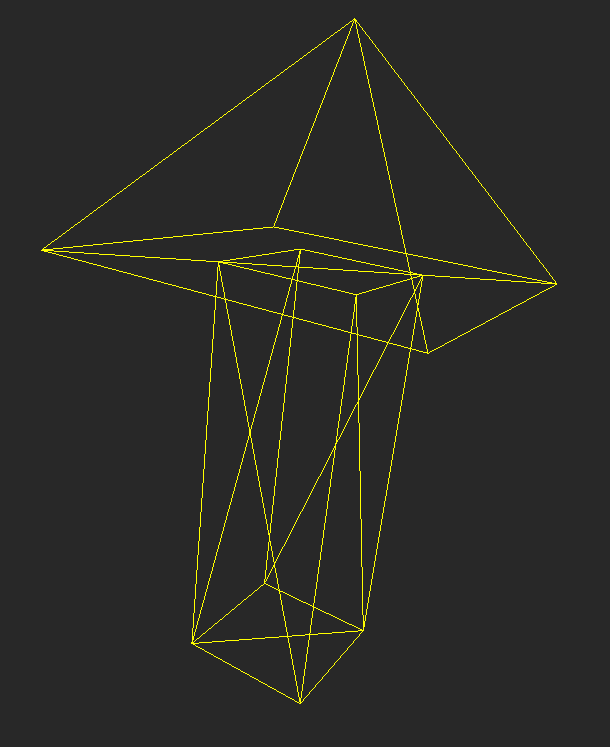
\includegraphics[width=\textwidth]{./img/4sided_arrow.PNG}
    \caption{Four-sided tip version (not used)}
    \label{fig:4sided_arrow}
	\end{subfigure}
    \qquad
    \begin{subfigure}{0.3\textwidth}
	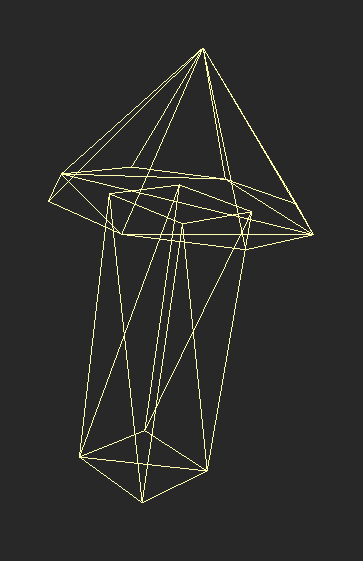
\includegraphics[width=\textwidth]{./img/8sided_arrow.PNG}
    \caption{Eight-sided tip version (used)}
    \label{fig:8sided_arrow}
	\end{subfigure}
\caption[Wireframe models used for arrow visualizations]{Wireframe models used for arrow visualizations}
\end{figure}

The visualizer receives a list of clusters as input, loops through those which passed through thresholding and makes a scaled copy of the basic arrow in each iteration. The scale of the copy is based on the representative vector of the cluster as described in section \ref{sec:analysis_visualizations}. A {\it scene} containing all the created copies is then outputted.

\subsubsection{Color Visualizers}

For each color visualization type mentioned in section \ref{sec:analysis_visualizations} (i.e. random, cluster relative, cluster absolute, etc.), there is a separate visualizer class implementing the color visualizer interface. This determines how color is assigned to vertices. In general, each visualizer loops though all \verb+Cluster+ instances supplied and for each of them it generates a color based on the metric value for that cluster. Clusters which were excluded in thresholding receive a special predefined color. Once a color is created, it is inserted into a list at precisely those indices which belong to the \verb+PrimaryArrows+ (see section \ref{sec:implementation_clustering}) of the associated cluster in the underlying {\it scene}. It is important to respect this indexing in order to make the mapping of the colors to the mesh vertices easier in the \verb+BakeVisualization()+ method of the \verb+DiffVector+ class. This list is then outputted.

It it worth mentioning that we have also implemented color visualizers which ignore the representative vectors of clusters and use the \verb+PrimaryArrows+ field of a \verb+Cluster+ instance to create vertex color visualizations similar to the ones presented in section \ref{sec:existing_visualizations}. Even though a similar effect can be achieved when the ``empty'' clustering is used, this approach works regardless of the clustering type selected. This means that a combined visualization can be created where arrows are clustered but colors are not\footnotemark.

\footnotetext{As mentioned at the beginning of section \ref{sec:implementation_clustering}, one \verb+DiffVector+ instance which controls the whole visualization process can only use a single type of clustering. We have made this decision to save data because if more types were allowed, more dendrograms would have to be stored in memory. Also, we have not found it very useful to combine clustering types in any other way than the one presented here.}

\subsubsection{Output}

Either a triangle mesh or a list of triplets representing colors is outputted based on the type of the visualization.
%%-----------------------------------------------------------------------------------------
\subsection{Visualization Output}
\label{sec:implementation-visualizers-output}

Lastly, we will mention how generated visualizations can be obtained through the \verb+BakeVisualization()+ method of \verb+DiffVector+ after \verb+CreateVisualization()+ has been called.

When two {\it scenes} in a specific order are provided to \verb+BakeVisualization()+, several actions might be performed based on which visualizations are available in \verb+DiffVector+:

\begin{itemize}
\item If a color visualization is available, the scenes are assumed to be the {\it primary scene} and the {\it reference scene} that the visualization was computed for, respectively, and all vertices of the scenes are assigned the corresponding color. For the {\it primary scene}, colors are assigned as they are in the visualization. For the {\it reference scene}, all colors are inverted because from the perspective of the {\it reference scene} the original metric vectors point in the opposite direction.
\item If an arrow visualization is available, the whole {\it scene} of arrows (see section \ref{sec:implementation_visualizers} for more details) is copied into the supplied {\it scenes}, where the assumed {\it reference scene} receives inverted arrows.
\item If both are available, the color visualization is baked first because the number of colors and {\it scene} vertices would not match after the arrow visualization was baked.
\end{itemize}

It is noteworthy that in the second case, there are no assumptions on the supplied {\it scene}, therefore it can be empty, in which case arrows are stored separately from the underlying {\it scene} for greater flexibility, or it can be either the {\it primary} or the {\it reference} scene, in which case everything is stored in one data structure.

Because both the {\it primary scene} and the {\it reference scene} are assigned a visualization, they can be displayed next to each other in order to emphasize the effect of the visualization. We will talk about this and the overall architecture of MeshDiff in the next chapter.
%%-----------------------------------------------------------------------------------------
%% SECTION
%%-----------------------------------------------------------------------------------------
\section{MeshDiff Architecture}

Similarly to MeshLab or Morphome3cs, in MeshDiff, the core functionality is the ability to load and store triangle meshes and to view them interactively using the mouse cursor. Because this functionality is present in almost all programs which work with triangle meshes and at the same time it is non-trivial, we reused available code which provides it, more specifically we built MeshDiff on top of a mesh viewer application written by Josef Pelikán.

%%-----------------------------------------------------------------------------------------
\subsection{Platform}

The reused code by Josef Pelikán is a C\# application with a WinForms user interface which uses the OpenTK library, which encapsulates the OpenGL API, to render graphics. This means that the only targeted operating system is Windows.

In order to clearly mark which parts of MeshDiff are authored by us and which are reused, we have stated the origin of the code in each source file and in this thesis, we will use the terms {\it resued code} and {\it original code} to differentiate between the two.

%%-----------------------------------------------------------------------------------------
\subsection{Triangle Mesh Viewing}

The {\it reused code} of MeshDiff supports two standard triangle mesh formats, \verb+.obj+ and \verb+.ply+. It is able to load and store files in these formats and also convert between them and the internal {\it scene representation} (see section \ref{sec:mesh_representation}) of a triangle mesh. The {\it scene} can be prepared for rendering by storing its data in the vertex buffer object in the GPU. This can be accomplished by calling one of its own methods. In each frame, a rendering method is called which comprises OpenTK calls tied to a view panel showing the triangle mesh. The view panel is a custom OpenTK control placed directly in the main form of the application. This process can be configured by a set of toggles which can change the viewing mode to wireframe, enable shading, etc.

Interactivity is handled by a class called \verb+Trackball+ which intercepts mouse events from the user interface and modifies the model matrix used in the rendering process.

We have added several modifications to this basic setup to support the rendering of visualizations of the difference between two triangle meshes. Here are the most significant ones:

\begin{itemize}
\item We have added a second viewing panel for the inverted visualization on the {\it reference mesh}. This required duplicating the buffer objects, \verb+Trackball+ instances and also fields which stored the loaded {\it scenes}.
\item Based on that we have added the option to either control both views separately, or to control both of them at the same time. This is done be routing the mouse events from the view panels either to both \verb+Trackball+ instances or only the intended one.
\item As mentioned in section \ref{sec:implementation-visualizers-output}, when 3D arrows are part of the visualization, they can be stored and loaded separately. For this case, we have added the option to toggle wireframe view independently for both displayed scenes. We therefore have separate fields for {\it scenes} containing arrows and more buffer objects to store them on the GPU.
\item Lastly, the user is able to hide the computed visualizations and show the original triangle meshes instead. Visualization {\it scenes} and raw {\it scenes} are therefore stored separately for these actions to happen quickly. Also, rendering methods now are now more flexible to make the transition between rendering various {\it scenes} easier.
\end{itemize}

%%-----------------------------------------------------------------------------------------
\subsection{User Interface}

We have extended the original user interface by adding functionality which allows the user to configure the visualization before it is generated. For the complete description of the configuration options, see appendix \ref{sec:parameter_description}. The user can also save this configuration to a file or load it from a file.

View configuration and the most important clustering and visualization parameters can be modified directly from the main form. Metric type and all other parameters have their separate dialog windows.

There are four places in the code where this configuration is held. The \verb+Trackball+ class remembers the model matrix and zoom value for each of the displayed triangle meshes. Currently chosen difference metric type is stored in a single variable. Clustering parameters (see section \ref{sec:parameter_effect}) have their own dedicated class and so do the visualization parameters which control the appearance of the visualizations.

Apart from being able to pass the parameters to the \verb+DiffVector+ class in a compact way, this approach also has the advantage that each class encapsulating a certain group of parameters is also able to write them to a file and it is also able to initialize itself from a file\footnotemark. For further details on this functionality, see appendix \ref{sec:parameter_load_store}.

\footnotetext{Metric type is stored in a variable but there is a dedicated class called \verb+Metric+ in the program which handles metric computation and on top of that is also able to handle the input/output operations.}

Each of the parameter classes implement individual parameters as properties and handle value checks. Exceptions thrown by these checks are not being caught, however, because the user interface is designed in such a way that invalid values cannot be assigned. Invalid assignments from code are then correctly detected and an exception is thrown in such cases.
%%-----------------------------------------------------------------------------------------
\subsection{Visualization Infrastructure}

Once the user has finished their configuration and started the visualization generation, an asynchronous job is initialized to handle this process in a user-friendly way.

The complete configuration including the visualizer classes (see section \ref{sec:implementation_visualizers}) and {\it scenes} visualization baking (see section \ref{sec:implementation-visualizers-output}) become part of a job configuration package. Once a job is initialized with this package, its behavior is fully determined and its \verb+Run()+ method can be assigned to a thread. A job operates directly with the \verb+DiffVector+ class, initializes it and calls its methods according to the configuration package. The thread is started together with a dialog window which shows progress and at the same time prevents the user from doing anything else with the program. Once the visualization process finishes, the program checks whether it has finished successfully or not and assigns based on that either renders the computed visualization {\it scenes} or reports an error and renders the raw {\it scenes}.
\chapter{Mesh Diff}

About the experimental application. (User documentation.)

\begin{itemize}
\item Talk about loading/saving parameters/visualizations
\end{itemize}
\chapter{Discussion}

In this chapter, we conclude the user study with a discussion of its results, strengths and weaknesses. In addition to that, we also include other observations and results based on the new visualizations.

\section{Study}

We cannot eliminate the possibility that the results of the study were influenced by the choice of data. We argue that humans are more sensitive 

\section{Visualizations}

\chapter*{Conclusion}
\addcontentsline{toc}{chapter}{Conclusion}


%%% Bibliography
%%% Bibliography (literature used as a source)
%%%
%%% We employ bibTeX to construct the bibliography. It processes
%%% citations in the text (e.g., the \cite{...} macro) and looks up
%%% relevant entries in the bibliography.bib file.
%%%
%%% The \bibliographystyle command selects, which style will be used
%%% for references from the text. The argument in curly brackets is
%%% the name of the corresponding style file (*.bst). Both styles
%%% mentioned in this template are included in LaTeX distributions.

\bibliographystyle{plainnat}    %% Author (year)
% \bibliographystyle{unsrt}     %% [number]

\renewcommand{\bibname}{Bibliography}

%%% Generate the bibliography. Beware that if you cited no works,
%%% the empty list will be omitted completely.

\bibliography{bibliography}

%%% If case you prefer to write the bibliography manually (without bibTeX),
%%% you can use the following. Please follow the ISO 690 standard and
%%% citation conventions of your field of research.

% \begin{thebibliography}{99}
%
% \bibitem{lamport94}
%   {\sc Lamport,} Leslie.
%   \emph{\LaTeX: A Document Preparation System}.
%   2nd edition.
%   Massachusetts: Addison Wesley, 1994.
%   ISBN 0-201-52983-1.
%
% \end{thebibliography}


%%% Figures used in the thesis (consider if this is needed)
\listoffigures

\begin{comment}

%%% Tables used in the thesis (consider if this is needed)
%%% In mathematical theses, it could be better to move the list of tables to the beginning of the thesis.
\listoftables

%%% Abbreviations used in the thesis, if any, including their explanation
%%% In mathematical theses, it could be better to move the list of abbreviations to the beginning of the thesis.
\chapwithtoc{List of Abbreviations}

\end{comment}

%%% Attachments to the bachelor thesis, if any. Each attachment must be
%%% referred to at least once from the text of the thesis. Attachments
%%% are numbered.
%%%
%%% The printed version should preferably contain attachments, which can be
%%% read (additional tables and charts, supplementary text, examples of
%%% program output, etc.). The electronic version is more suited for attachments
%%% which will likely be used in an electronic form rather than read (program
%%% source code, data files, interactive charts, etc.). Electronic attachments
%%% should be uploaded to SIS and optionally also included in the thesis on a~CD/DVD.
%%% Allowed file formats are specified in provision of the rector no. 72/2017.
\appendix
\chapter{Attachments}

%%-----------------------------------------------------------------------------------------
%% SECTION
%%-----------------------------------------------------------------------------------------
\section{Parameter Description}
\label{sec:parameter_description}

As mentioned in section \ref{sec:implementation_algorithm}, the proposed visualizations can be configured by a set of clustering parameters, a set of visualization parameters and a few other parameters. We will now provide an overview of all of them.

%%-----------------------------------------------------------------------------------------
\subsection{Clustering Parameters}
\label{sec:clustering_parameters}

\begin{description}
\item [Cluster Count] Determines the number of clusters to be retrieved from the dendrogram (see Fig. \ref{fig:telea-hierarchical_clustering}) and used for visualization. If the dendrogram is a tree, any valid number of clusters is guaranteed to cover the whole data set. If the dendrogram is a forest (see section \ref{sec:analysis_clustering_algorithm}), certain parts of the data set may remain uncovered by the chosen clusters. {\bf Valid values:} \(\bm{[1,S]}\) where \(S\) is the number of vertices of one of the {\it scenes}.
\item [Direction Significance] Determines how large the direction weight coefficient in the error function (see Eq. \ref{eq:clustering_error}) will be. See section \ref{sec:parameter_effect} for details. It is only meaningful in combination with all the other significance parameters\footnotemark. {\bf Valid values:} \(\bm{[0,100]}\)
\item [Magnitude Significance] Determines how large the magnitude weight coefficient in the error function (see Eq. \ref{eq:clustering_error}) will be. See section \ref{sec:parameter_effect} for details. It is only meaningful in combination with all the other significance parameters\footnotemark. {\bf Valid values:} \(\bm{[0,100]}\)
\item [Position Significance] Determines how large the position weight coefficient in the error function (see Eq. \ref{eq:clustering_error}) will be. See section \ref{sec:parameter_effect} for details. It is only meaningful in combination with all the other significance parameters\footnotemark. {\bf Valid values:} \(\bm{[0,100]}\)
\item [Resolution Significance] Determines how large the mesh resolution weight coefficient in the error function (see Eq. \ref{eq:clustering_error}) will be. See section \ref{sec:parameter_effect} for details. It is only meaningful in combination with all the other significance parameters\footnotemark. {\bf Valid values:} \(\bm{[0,100]}\)
\end{description}

\addtocounter{footnote}{-4}
\stepcounter{footnote}\footnotetext{\label{conversion}Here is the conversion between {\it significance} and {\it weight}: Consider {\it significance} values \(s_d,s_m,s_p,s_r \in [1,100]\) and {\it weight} values \(k_d,k_m,k_p,k_r \in [0,1]\). We need \(k_d + k_m + k_p + k_r = 1\), therefore \(k_d = s_d / {(s_d + s_m + s_p + s_r)}\) and similarly for all other weights.}
\stepcounter{footnote}\footnotetext{See footnote \ref{conversion}.}
\stepcounter{footnote}\footnotetext{See footnote \ref{conversion}.}
\stepcounter{footnote}\footnotetext{See footnote \ref{conversion}.}

%%-----------------------------------------------------------------------------------------
\subsection{Visualization Parameters}
\label{sec:visualization_parameters}

\begin{description}
\item [Arrow Height Minimum Scale] Determines the height of an arrow representing the lowest metric value present in the data set. This value will multiply the height of the default arrow (see section \ref{sec:implementation_visualizers}) and therefore does not represent the absolute value of the minimum arrow height. {\bf Valid values:} \(\bm{[0.1,10]}\)

\item [Arrow Height Maximum Scale] Determines the height of an arrow representing the highest metric value present in the data set. This value will multiply the height of the default arrow (see section \ref{sec:implementation_visualizers}) and therefore does not represent the absolute value of the maximum arrow height. {\bf Valid values:} \(\bm{[0.1,10]}\)

\item [Arrow Width Minimum Scale] Determines the width of an arrow representing a cluster with the smallest area out of all visualized clusters. This value will multiply the width of the default arrow (see section \ref{sec:implementation_visualizers}) and therefore does not represent the absolute value of the minimum arrow width. {\bf Valid values:} \(\bm{[0.1,10]}\)

\item [Arrow Width Maximum Scale] Determines the width of an arrow representing a cluster covering the whole data set. This value will multiply the width of the default arrow (see section \ref{sec:implementation_visualizers}) and therefore does not represent the absolute value of the maximum arrow width. {\bf Valid values:} \(\bm{[0.1,10]}\)

\item [Arrow Outwards Color] Determines the color of arrows pointing {\it outwards} (see section \ref{sec:analysis}). {\bf Valid values: Any RGB color}.

\item [Arrow Inwards Color] Determines the color of arrows pointing {\it inwards} (see section \ref{sec:analysis}). {\bf Valid values: Any RGB color}.

\item [Color Metric Outwards] Determines the hue of vertices which are assigned a metric vector pointing {\it outwards} (see sections \ref{sec:analysis} and \ref{sec:analysis-color}). {\bf Valid values: Any RGB color}.

\item [Color Metric Inwards] Determines the hue of vertices which are assigned a metric vector pointing {\it inwards} (see sections \ref{sec:analysis} and \ref{sec:analysis-color}). {\bf Valid values: Any RGB color}.

\item [Color Diff Threshold] In absolute mode (see section \ref{sec:analysis-color})), all vertices with an associated metric vector longer than this value will receive the brightest color. {\bf Valid values:} \(\bm{[1, \infty)}\) (In the MeshDiff UI this is limited by the diameter of the whole scene.)

\item [Disabled Color] The color of vertices which were excluded from the visualization by thresholding. {\bf Valid values: Any RGB color}.

\item [Disabled Threshold Length] All vertices with a shorter associated metric vector will be excluded from the visualization. {\bf Valid values:} \(\bm{[1, \infty)}\) (In the meshDiff UI this is limited by the diameter of the whole scene.)

\item [Disabled Threshold Size] All vertices which are part of a cluster whose area is smaller than this value will be excluded from visualization. {\bf Valid values:} \(\bm{[1, \infty)}\) (In the meshDiff UI this is limited by the diameter of the whole scene squared.)
\end{description}

%%-----------------------------------------------------------------------------------------
\subsection{Other Parameters}

The rest of the parameters comprise the viewing angle and zoom of both {\it scenes} and also the metric type, clustering type and visualization type. They are used to configure the mesh viewer in MeshDiff and they also determine how the \verb+DiffVector+ class is initialized (see section \ref{sec:implementation-framework}).

\begin{description}
\item [Zoom Left \& Right] Determines the zoom factor of the mesh view. {\bf Valid values: Not limited.} (The default value is 1.)
\item [Rotation Left \& Right] Determines the viewing angle of a mesh. {\bf Valid values: Any 4x4 rotation matrix.}
\item [Metric] Determines the metric type used in difference computation. (See section \ref{sec:analysis}.) {\bf Valid values: \{Distance, NormalProjectedDistance\}}
\item [Clustering Type] Determines the type of clustering used in the visualization process. (See section \ref{sec:implementation_clustering}.) {\bf Valid values: \{None, Simple, Signed\}}
\item [Color Visualization] Determines the type of color visualization used. (See section \ref{sec:analysis-color}.) {\bf Valid values: \{None, VertexRelative, VertexAbsolute, ClusterRandom, ClusterRelative, ClusterAbsolute\}}
\item [Arrow Visualization] Determines whether arrow visualization is used. {\bf Valid values: \{True, False\}}
\end{description}

%%-----------------------------------------------------------------------------------------
%% SECTION
%%-----------------------------------------------------------------------------------------
\section{Parameter Loading and Storing}
\label{sec:parameter_load_store}

In this section, we describe how MeshDiff can write its configuration to a file and also read it from a file. First, we will talk about the file format. It is a very simple custom format designed to store key/value pairs and to allow for easy reading and writing. Then we will mention how the process of reading and writing is realized in the code.

%%-----------------------------------------------------------------------------------------
\subsection{Format}

Each file is divided into sections which are delimited by a special line containing the name of the section. What follows are key/value pairs, one pair per line. Here is an example of a full configuration file:

\begin{code}
---Trackball Left---
zoom=1
rotation=1,0,0,0;0,1,0,0;0,0,1,0;0,0,0,1

---Trackball Right---
zoom=1
rotation=1,0,0,0;0,1,0,0;0,0,1,0;0,0,0,1

---Metric---
metric=distance

---Clustering Parameters---
clusterCount=20
directionSignificance=15
positionSignificance=25
magnitudeSignificance=10
resolutionSignificance=0

---Visualizer Parameters---
arrowColorNear=0.5019608,0.5019608,0
arrowColorFar=0.5019608,0.5019608,0
colorNear=0.5019608,0,0.5019608
colorFar=0.5019608,0,0.5019608
disabledColor=1,0.5019608,0
arrowWidthMinScale=10
arrowWidthMaxScale=10
arrowHeightMinScale=10
arrowHeightMaxScale=10
disabledThresholdLength=0.3
disabledThresholdSize=0.8
colorDiffThreshold=0.1

---Form Settings---
clusteringType=None
colorVisualization=None
arrowVisualization=False
\end{code}

All lines which do not fulfill any of the following requirements are ignored:

\begin{itemize}
\item Start with \verb+---+
\item Yield exactly two strings upon split at \verb+=+
\end{itemize}

The format of keys and values is defined by the program.
%%-----------------------------------------------------------------------------------------
\subsection{Loading and Storing}

We have written \verb+ParameterWriter+ and \verb+ParameterReader+ classes which can be used in a similar way other I/O classes are used in C\#.

\verb+ParameterReader+ is initialized with a file path and a section name which is the full delimiting string shown above. Then a \verb+ReadPair()+ method can be called in a loop and key/value pairs are returned as tuples. When there are no more pairs in the given section, \verb+null+ is returned. All objects of this class should be disposed of at the end of their lifetime.

\verb+ParameterWriter+ is also initialized with a file path and a section name and provides two methods: \verb+WritePair()+ and \verb+WriteEmptyLine()+. Both methods write to the given file and they always append to file. Upon the first call, a section of the given name is created and all subsequent calls write key/value pairs under that section. \verb+WritePair()+ can only accept arguments of type \verb+string+. This class also implements the \verb+IDisposable+ interface.

\openright
\end{document}
